\documentclass[11pt]{article}
\usepackage[utf8]{inputenc}
\usepackage[english]{babel}
\usepackage{aas_macros}
\usepackage{hyperref}
\usepackage{appendix}
%\usepackage[hmargin=1.5cm, vmargin=0.55cm]{geometry}
\usepackage[hmargin=1.5cm, vmargin=1.5cm]{geometry}
\usepackage{amsmath}
\usepackage{caption}
\usepackage{mathtools}
\usepackage{fancyhdr}
\usepackage{float}%Places the float at precisely the location in the LaTeX code...i.e, [H]
\usepackage{wrapfig}
\usepackage{rotating}
\usepackage{pdfpages}

%for quotes
%\epigraphfontsize{\small\itshape}
%\setlength\epigraphwidth{8cm}
%\setlength\epigraphrule{0pt}


%\usepackage[pdftex]{graphicx}%includegraphics
%converts eps to pdf
\usepackage[update,prepend]{epstopdf}
%\usepackage{subcaption} %need to find subcaption.sty for this to work!
%\usepackage{epstopdf}
\newcommand{\Lagr}{\mathcal{L}}
%\graphicspath{ {~/PhD/Thesis/upgrade-plots/} {./} }
\DeclareGraphicsExtensions{.pdf,.png,.jpg,.eps,.gif,.ps}
\renewcommand{\vec}[1]{\mathbf{#1}}
\usepackage[round]{natbib}  %use the "Natbib" style for the references in the Bibliography
%\usepackage{aastex}%defines journal abbreviations in bib file
%\newcommand{name}[num]{definition}



%\title{Lower Atmospheric Signatures During Solar Flares \\ Associated with Seismicity}
%\author{Jamie Ryan \\
%Mullard Space Science Laboratory \\
%University College London \\
%Surrey, RH13 6NL, UK\\
%\href{mailto:jamie.ryan.14@ucl.ac.uk}{jamie.ryan.14@ucl.ac.uk}
%\date{}}

%\pagestyle{headings}
%\setcounter{page}{1}

\begin{document}
\includepdf{upgrade-title-page}
\pagenumbering{roman}
\tableofcontents

%%%%%%%%%%%%%%%%%files containing bodies of text%%%%%%%%%%%%%%%%%%
%%%%%%%%%%%%%%%%%%%%%%%%%%%%%%%%%%%%%%%%%%%%%%%%%%%%%%%%%%%%%%%%%%
%%%%%%%%%%%%%%%%%%%%%%%%%%%%%%%%%%%%%%%%%%%%%%%%%%%%%%%%%%%%%%%%%%
%\begin{abstract}
Sunquakes represent the propagation of acoustic waves in the sub-photosphere, responding to an excitation of the photosphere during the impulsive phase of solar flares. The progenitors of sunquakes are thought to be either shocks, radiative backwarming, direct particle collision or sudden magnetic field reconfiguration. Each of these mechanisms relies on the transport of energy from the corona to the photosphere, and the physical conditions existing in the chromosphere such as magnetic configuration and density. To understand sunquakes and their relationship to solar flares, we need to understand how energy moves down through the solar atmosphere and the physical conditions that are present. An X1 solar flare with associated sunquake was observed in active region NOAA 12017 on the 29th of March 2014 at 17:46 UTC, by multiple spacecraft, including SDO (HMI), IRIS and RHESSI. Lightcurves of the flare emission from the photosphere, chromosphere and transition region are analysed providing information about the deposition of energy at different altitudes in the solar atmosphere. Hard X-ray footpoints of coronal loops are shown to align well with an area associated with maximum acoustic power. Balmer continuum emission aligned with maximum acoustic power is shown to increase during the flare, indicating the existence of hydrogen recombination continua in the chromosphere possibly leading to radiative backwarming of the photosphere. 
\end{abstract}

%%Mark says: This should describe the aims of your research study and why the research problem is important. It should also set the scene for everything that follows.

%Lucie says: 
%*Fact check my %mythology, %science-history and %modern-day-view paragraphs.
%*Fusion
%*Structure
%*Energy transport from core to photosphere
%*Atmosphere (show classic T, rho plot)
%*Magnetic field (permeates entire Sun ands atmosphere)
%   *a couple of statements about internal dynamo
%   *field transported by ("frozen-in") bouyant plasma in the convection zone (flux tubes created by dynamo)
%   *Sunspots to coronal loops
%*Magnetic activity
%   *reconnection
%   *cme
%   *flares   
%*Sunquakes
%*My science question

\section{Introduction}

\epigraphfontsize{\small\itshape}
%insert quote
\epigraph{``So you run and you run to catch up with the sun but it's sinking \\
Racing around to come up behind you again. \\
The sun is the same in a relative way but you're older, \\
Shorter of breath and one day closer to death."}{--- \textup{Roger Waters} Time, Darkside of the Moon, Pink Floyd}


%mythology (pre-science)
Early scrawlings on cave walls and writings by later societies show that the Sun has been an object of mystery and mythology for much of human history. Many pre-scientific civilisations worshipping this all powerful bringer of life, often in the form of a female deity. For instance, Norse society beleived that the Sun or Sól, rode her horse drawn chariot through the sky, in a daily race against pusuing darkness which has taken the form of ravenous wolves. It was thought that if Sól was overtaken by these dark wolves then cosmic chaos would insue, with the end result being the destruction of all that humans and the gods held dear. This particular fable shows how the Sun has been interwoven in to our explanation of the world around us, with, "what if the Sun does not rise?" being one of our oldest philisophical questions. To some extent it is thought that, such beliefs still permeate todays society, in fact, theologan scholars speculate that many of the modern forms of religion are probably the result of a rewriting of solar mythology.  


%science history
Other than being held as an all powerful omnipitant being, the Sun has fascinated inquisitive minds for much of history and there are documented examples of solar study, going back thousands of years. From as early as 2000 B.C., the Chinese were able to predict when a solar eclipse would occur. Moving forward around 1500 years to 350 B.C., and some of the first sunspot observations are made by Aristotles student, Theophrastus. These early examples of the Sun occupying the minds of the days critical thinkers surely makes the study of the Sun one of the oldest scientific pursuits.      


%modern day view
In comparison, scientists today have an exquisitely detailed, spaceborn view of the Sun. This has lead to an understanding of many of the physical processes that dictate the dynamics and life cycle of our parent star. It is now accepted that the Sun is a 4.5 billion year old G-type, main sequence star in a state of hydrostatic equilibrium. Powered by nuclear fusion, the Sun emits around $3.86\times10^{26}$ $ Joules of energy per second, which is enough to meet the world's annual power consumption a million times over. This energy is generated in the solar core, by nuclear decays that lead to chain reactions, releasing photons that can take approximately 100,000 years to travel from the core to the photosphere. The Sun is able to fuse atoms in this way because of the huge pressures generated within the core caused by the strong gravitational field. The Sun and all main sequence stars are in a state of hydrostatic equilibrium, whereby outward gas pressure is balanced by the gravity generated by the stars mass. At some point, probably in around 4.5 billion years, the Sun will start to run out of Hydrogen fuel, at which point nuclear fusion in the core will cease. The gravitation field will be weakened due to this lack of mass in the core. Once the Sun's gravity is too weak to resist internal gas pressure the star will start to expand and eventually shed it's outer layers forming a planetary nebula.


So, other than nurturing the intelligent life that occupies this planet, the Sun is one unspectactular star in a 100 billion that make up our galaxy.


 %Introduction
%\section{Sunquakes}
\subsection{Introduction}
%Chronological soft intro; use some of the lit review,
%making sure to emphasize the connection to solar flares;Look at early papers predicting sunquakes(Wolff 70s and Kosovichev and Zharkova);the importance of sunquakes


During this age of space-born solar astronomy, understanding the highly dynamic environment of the Sun's atmosphere is a study enriched by a wealth of high detail observations. With each newly launched space instrument the spatial resolution of collected data increases, which coupled with those spacecraft that are tailored to capture light of previously unobserved wavelengths, often leads to new phenomena being observed. Eruptive solar flares fall into this category, in that spacecraft have provided observations that challenge the current theoretical view that the standard eruptive flare model (CSHK model: \citep{1964NASSP..50..451C, 1966Natur.211..695S, 1974SoPh...34..323H, 1976SoPh...50...85K} puts forward. 

Solar flares are one of the most energetic events to occur in the Sun's atmosphere, where by stored magnetic energy is released in the form of heat, mass motions, and accelerated particles. This highly dynamic process produces many measurable signatures, such as emission from $\gamma$-ray to optical wavelengths, a high percentage of which agree with the CSHK model, however, this is not the full picture. The standard flare model has been modified to include new observations many times over the years \citep{2011LRSP....8....6S} and is still unable to describe some observed phenomena. Therefore there is still work to be done before a true account of the complex nature of solar flares are to be realised.    

Sunquakes are an observable feature during some solar flares that the standard model is unable to explain. It is believed that they are the result of energy and momentum released during the flare impacting the lower solar atmosphere. During a solar flare, energy is released high up in the solar atmosphere and transported down to lower altitudes. If a sufficient amount of energy impacts the lowest atmospheric layer, then acoustic waves are produced which propagate into sub-surface layers of the Sun producing a sunquake (see figure \ref{sunquake-cartoon}a). As acoustic wave-fronts travel into the interior they encounter layers of increasing density causing refraction back toward the solar surface (see figure \ref{sunquake-cartoon}b). At which point, waves can be observed as circular formations in the surface plasma , expanding outward from a point of origin (see Figure \ref{mdiquake96}). 


\begin{figure}[hb]%\label{sunquake-cartoon}
  \begin{center}
  \includegraphics[width=0.99\textwidth]{sunquake-cartoon}
  \caption{Sunquake cartoon: a) Shows a basic picture of sunquake production. Energy moves down through the solar atmosphere impacting the photosphere and generating a sunquake. b) Shows acoustic wave-fronts propagating into the interior of the Sun. Wave-fronts refract back toward the surface as they encounter increasingly dense sub-surface layers. Waves reaching the surface disturb material in a pattern resembling ripples in a pond.}\label{sunquake-cartoon}
\end{center}
\end{figure}

\subsection{Sunquake Observations}
The possibility that solar flares cause acoustic waves inside the Sun was originally put forward by \citep{1972ApJ...176..833W}. Wolff made the connection that a large solar flare releasing enough energy to heat the photosphere, would generate expansion of photospheric material, which could lead to an impulsive stimulation of oscillations in the Sun's interior. Wolff also commented that it would be difficult to observe interior oscillations with current solar velocity measurement techniques.      

A little over twenty years later and Wolff's idea was built upon by \cite{1995ESASP.376b.341K}, who showed theoretically that acoustic waves in the solar interior could be generated by a large solar flare, and that they may be detectable. A year later and the first detection of a sunquake was made by \cite{1998Natur.393..317K} during an X class solar flare on July the 9th 1996. Their observational data came from the Solar and Heliospheric Observatory (SOHO) via the Michelson Doppler Imager (MDI) which images the movement of photospheric material by analysing shifts in wavelength of the emitted light. They observed a prominent impulsive downward signature in the Dopplergrams directly over a compact point source emanating a set of concentric acoustic waves (see Figure \ref{mdiquake96}. The timing of maximum downward velocity of material derived from the Dopplergrams was out of sync with peak hard x-ray measurements by around a minute. This time delay, coupled with white-light enhancement in the lower atmosphere led to the conclusion that during the flare, accelerated energetic particles heat the cool dense chromosphere causing a shock front which travels downward, depositing energy in lower atmospheric layers, generating a sunquake. 
 
\begin{figure}[hb]
  \begin{center}
  \includegraphics[width=0.80\textwidth]{soho-mdi-quake-96}  
\caption{\cite{1998Natur.393..317K} produced SOHO MDI Dopplergrams from the 1996 July 9th, X class solar flare showing the sunquake expanding outward from it's seismic epicentre to a radial distance of $1.2\times10^{8}$ metres. Wave-fronts accelerate from a velocity of 30km/s to 100km/s}\label{mdiquake96}
\end{center}
\end{figure}


The first sunquake observation opened up a whole new area of solar physics to science, leading to a multitude of detections associated with many different flares. The majority of observations show that sunquakes are often the product of highly impulsive flares, with the acoustic source aligning spatially with white light enhancement in the lower solar atmosphere and hard x-ray emission from the upper-atmosphere \citep{2005ApJ...630.1168D, 2007ApJ...664..573Z}. \cite{2005ApJ...630.1168D} went on to calculate the energy needed to stimulate the propagation of an acoustic wave in the sub-photosphere. The authors found that only $\sim10^{-3}$ of the energy released by a flare is enough to generate a sunquake. This was an important calculation because it forced the solar community to consider that it might be possible for smaller energy flares to produce sunquakes, leading subsequent work (e.g., \cite{2008SoPh..251..613M}) analysing sunquakes from lower energy flares.

A paper by \cite{2000ApJ...531L..75H} put forward for the first time, that sunquake production may depend on the changing configuration of the magnetic field. This idea was further reinforced by \cite{2001ApJ...550L.105K} reporting observations of impulsive changes in magnetic field strength at the photosphere during a solar flare. These magnetic transients were shown to approximately correlate in time and space with hard x-rays and impulsive increases in plasma velocity and emission intensity. This line of study was continued \citep{2009MNRAS.395L..39M}, investigating the magnetic field variation of the photosphere in many flares. The study found that some flares with seismicity do not have a spatial and temporal correlation between sunquakes and magnetic transients. Some flares have magnetic transients and no seismicity, and some flares have a good co-spatial alignment of acoustic activity and magnetic variability. It was noted that the impulsiveness of the magnetic field variation could be important as to whether a sunquake is generated.

Probably the most intriguing of sunquake observations are those that do not abide by the usual set of observable features, in that they are not necessarily associated with hard x-rays and white-light emission. For example, a statistical survey carried out by \cite{2012SoPh..277..317P}, highlighted a flare containing three footpoints with a seismic source that was co-temporal but not co-spatial with it's closest HXR footpoint; and another source which was co-spatial and co-temporal with it's nearest HXR footpoint.

Another example by \cite{2011ApJ...741L..35Z} reports an observation of two seismic sources associated with a flare that erupts producing a coronal mass ejection (CME). During the eruption, the magnetic field above each seismic source undergoes an abrupt permanent reconfiguration. The authors cite the possibility that there exists particle beams low enough in population that HXR emission is undetectable. Further papers investigating the same event \citep{2013SoPh..284..315Z} showing that there are downward motions of material above the seismic sources and that energy provided by magnetic transients may not be able to account for the acoustic power generated.       

\subsubsection{Sunquake Progenitors}\label{sunprog}
%list and explain current theories of sunquake generation
%making sure to highlight the different observables that can identify each mechanism, eg wlf = evidence of radiative backwarming  


The progenitors of sunquakes are still unknown and as a result this is an exciting area of research with discoveries still to be made. The general consensus, in terms of valid mechanisms that could cause this phenomenon is an area of contention, however the following progenitors are thought to be at least partly responsible. \\

\begin{itemize}
\item \textbf{Radiative backwarming} as a mechanism for producing sunquakes, was first put forward by \cite{2005ApJ...630.1168D} to account for a spatial correlation between seismic sources and white light emission from the lower atmosphere. The idea is that during a solar flare, high energy electrons and photons impulsively heat the photosphere producing white light emission \citep{1989SoPh..124..303M}. This causes an increase in radiation pressure in the photosphere which causes acoustic waves to propagate into the sub-photosphere. \\
     
\item \textbf{Sudden magnetic field reconfiguration} was first detailed by \cite{2008ASPC..383..221H}. Solar flares are violent physical processes that involve the evolution of magnetic fields and charged solar plasma. Due to the Lorentz force, it is possible for a magnetic field to impart a force on a charged material and vice versa. If, during a solar flare, the magnetic field close to the photosphere relaxes to a more horizontal alignment it can impart a force on the photospheric material resulting in the production of acoustic waves, which propagate into sub-photosphere. The key parameter for this mechanism seems to be that the field has to reconfigure in an sufficiently impulsive manner to generate enough force to induce seismic waves. \\

\item \textbf{Shocks} are a mechanism originally proposed in initial work by \cite{1995ESASP.376b.341K} and \cite{1998Natur.393..317K}, whereby a shock wave propagates from the upper-chromosphere down to the photosphere generating sub-photospheric acoustic waves. During a solar flare, particles and heat are directed down toward the chromosphere, at which point chromospheric material reacts with and increase in temperature. This increased temperature causes explosive ablation of chromospheric material both upward and downward. The downward component develops into a shock front carrying energy to the lower atmosphere, which can go on to heat the photosphere causing radiative backwarming \citep{1989SoPh..124..303M}. \\

\item \textbf{Direct proton collision}, is linked to observations by \cite{2007ApJ...664..573Z} where the sunquake was spatially aligned with $\gamma$-ray emission. $\gamma$-rays during a solar flare are an indicator of energetic protons being accelerated along a newly reconfigured magnetic field. Proton beams carry more momentum than electron beams and are able to penetrate into the lower atmosphere, depositing energy in the form of heat. If an energetic beam of protons makes it down to the photosphere, it can cause radiative backwarming \citep{1989SoPh..124..303M}, which in turn causes the sunquake as described above. \\

\end{itemize}

 %Introduction

%Mark says: This should describe the aims of your research study and why the research problem is important. It should also set the scene for everything that follows.

%Lucie says: 
%*Fact check my %mythology, %science-history and %modern-day-view paragraphs.
%*Fusion
%*Structure
%*Energy transport from core to photosphere
%*Atmosphere (show classic T, rho plot)
%*Magnetic field (permeates entire Sun ands atmosphere)
%   *a couple of statements about internal dynamo
%   *field transported by ("frozen-in") bouyant plasma in the convection zone (flux tubes created by dynamo)
%   *Sunspots to coronal loops
%*Magnetic activity
%   *reconnection
%   *cme
%   *flares   
%*Sunquakes
%*My science question

\section{Introduction}
%Chronological soft intro; use some of the lit review,
%making sure to emphasize the connection to solar flares;Look at early papers predicting sunquakes(Wolff 70s and Kosovichev and Zharkova);the importance of sunquakes
During this age of space-born solar astronomy, understanding the highly dynamic environment of the Sun's atmosphere is a study enriched by a wealth of high detail observations. With each newly launched space instrument the spatial resolution of collected data increases, which coupled with those spacecraft that are tailored to capture light of previously unobserved wavelengths, often leads to new phenomena being observed. Eruptive solar flares fall into this category, in that spacecraft have provided observations that challenge the current theoretical view that the standard eruptive flare model (CSHKP model: \citep{1964NASSP..50..451C, 1966Natur.211..695S, 1974SoPh...34..323H, 1976SoPh...50...85K} puts forward.

Solar flares are one of the most energetic events to occur in the Sun's atmosphere, where by stored magnetic energy is released in the form of heat, mass motions, and accelerated particles. This highly dynamic process produces many measurable emission signatures at wavelengths from $\gamma$-rays to radio waves. Many of these observed signatures agree with the CSHKP model, however, this is not the full picture. The standard flare model has been modified to include new observations many times over the years (e.g., \cite{2011LRSP....8....6S}) and is still unable to describe some observed phenomena. 

Sunquakes are an observable feature during some solar flares that the standard model is unable to explain. It is believed that they are the result of energy and momentum released during the flare impacting the lower solar atmosphere. If a sufficient amount of momentum is imparted on the lowest atmospheric layer, then acoustic waves or 'sunquakes' are produced. The challenges presented in studying this phenomena are mainly associated with the ambiguous nature of the mechanism by which sunquakes are generated. Many ideas for the sunquakes progenitors have been put forward but at this point in time observable signatures do not always show a clear cut evidence aligning with current theories. Therefore this is an exciting time to be investigating the formation mechanisms of sunquakes and could also contribute to our overall understanding of solar flares.      
%%%%%%%%%%%%%%%%%%%%%%%%%%%%%%%%%%%%%%%%%%%%%%%%
%%%%%%%%END OF SOFT INTRO%%%%%%%%%%%%%%%%%%%%%%%
\subsection{Solar Atmosphere}
The solar atmosphere can be described as having four components, the corona, transition region, chromosphere and photosphere, see Figure \ref{solatmpics}.

\begin{figure}[H]%\label{sunquake-cartoon}
  \begin{center}
  \includegraphics[width=0.20\textwidth]{2014_03_29_17_19_42_HMI_Int}%photsphere
  \includegraphics[width=0.20\textwidth]{2014_03_29_17_19_42_AIA_304}%chromosphere
  \includegraphics[width=0.20\textwidth]{2014_03_29_17_19_42_AIA_171}%tr
  \includegraphics[width=0.20\textwidth]{2014_03_29_17_19_42_AIA_193}%corona
  \caption{ Images taken from the Solar Dynamics Observatory (SDO) instruments, the Helioseismic Magnetic Imager(HMI) and the Atmospheric Imaging Assembly (AIA) displaying the four main components of the solar atmosphere. From left to right layers of the solar atmosphere are increasing in altitude and temperature from the photosphere (SDO/HMI 6173 \AA\ continuum), to the chromosphere (SDO/AIA 304 \AA) through the transition region (SDO/AIA 171 \AA) then up to the corona (SDO/AIA 193 \AA). Images courtesy of \href{www.helioviewer.org}{www.helioviewer.org}}\label{solatmpics}
\end{center}
\end{figure}


For a sunquake to occur, energy released during a solar flare has to traverse these four layers propagating through many pressure scale heights as it does so. Pressure scale height is a measure of the distance over which pressure drops off by a factor of \emph{e}. For example, in the photosphere, $H\sim150$km, whereas in the corona, $H\sim100$Mm. Figure \ref{solatm} shows how the solar atmosphere changes with height, temperature and density, for each of the atmospheric layers. Information in this section is taken from text books: \cite{2003dysu.book.....D, 2004soas.book.....F}


\subsubsection{The Photosphere}
The photosphere is the lowest in altitude of the atmospheric layers, forming a shell around the Sun with a radius somewhere between $\sim10$ - $10^{2}$ km. With an effective temperature of $T\sim5800$K, the photosphere decreases in temperature with radial distance to $\sim4400$K in the temperature minimum region. Emission from this part of the atmosphere is predominantly in the visible range. Contained in the photosphere, are neutral hydrogen atoms, ions and electrons. When a neutral hydrogen atom captures a free electron it forms H$^{-}$ ions, which via absorption of UV and infrared radiation increases the opacity of the region. Even though it is thought that electron capture is a rare occurance, the population of H$^{-}$ ions is large enough to count for the majority of the photospheric opacity. The densest atmospheric layer, plasma pressure in the photosphere is domninant over magnetic pressure such that the plasma-beta, $\beta = p_{gas}/p_{mag} >> 1$. Because of frozen-in theorem (see section \ref{}) photospheric plasma dictates the motions of and to some extent, the morphology of the local magnetic field.

Granules are observed over almost the entire photosphere and are the physical representation of convection currents. Seen as the bright central part of the granule, bouyant, heated plasma rises from a region known as the convective zone, underneath the photosphere. As the material cools, it loses it's bouyancy and falls back toward the interior forming the darker areas surrounding the granule known as intergranular lanes.

Active regions on the photosphere contain sunspots, which are regions of intense magnetic field playing host to footpoints of loops that can extend out into interplanetary space. An active region is formed of at least two sunspots of opposing polarity. 
A sunspot is an approximately circular feature, made up of two main parts, the dark central umbra which is surrounded by the slightly lighter penumbra. The umbra hosts magnetic field lines that are tightly packed and pointing radially away from the Sun, whereas the penumbral magnetic field is more horizontal with respect to the solar surface. With a field strength of $\sim 10^{-1}$ Tesla, sunspots are regions in the photosphere where the magnetic pressure is dominant over plasma pressure, such that $\beta << 1$. Meaning that in these regions convection currents and radiative transfer are inhibited, with the latter being the idea behind a sunspot's dark appearance. \\


\subsubsection{Chromosphere}
The next region of the atmosphere is the chromosphere which is situated above the photosphere. This layer of plasma is a few thousand kilometres (2000 - 3000 km) thick and is optically thin to visible light so is difficult to observe against the brightness of the photosphere. The temperature in this layer increases with height from 4400 K at the temperature minimum region to $\sim10^{5}$K near the transition region. As a result, plasma density descreases and $\beta$ drops, crossing unity near the transition region between the upper-chromosphere and corona. This means that the pressure scale height in this region is changing with altitude as a transition from the plasma to magnetic domain occurs. The chromosphere is observable in the optically thick H$\alpha$ line in a red wavelength due to photoelectric processes. Whereas collisionally produced Ca II H & K and Mg II emission are observable in NUV wavelengths. Sunspots still exert enough influence to control chromospheric plasma and thus are still observable. In this region, dense material suspended in magnetic fields, or filaments, can be observed in absorption, or emission at the limb (prominence). Filaments are thought to be the source of mass for coronal mass ejections (CME) due to their location over active regions and a sudden emptying of material during eruptive flares with a CME. 

\subsubsection{Transition Region}
Up in altitude to the interface between the chromosphere and the corona or transition region. This region is a poorly understood layer of the solar atmosphere. What is known, is that; temperatures climb from $\sim10^{5}$ near the chromsphere to $\sim10^{6}$ K at the corona; this region has variable thickness and maybe even orientation; plasma density falls off sharply. This region can be observed in NUV wavelengths such as Si IV.  

\subsubsection{Corona}
The corona is the outer most layer of the atmosphere extending out into interplanetary space.  With a temperature ranging from $T\sim10^{6}$ - $10^{7}$ K, this the hottest part of the atmosphere. Plasma density in this region is very low, leading to a plasma pressure which is much lower than the magnetic pressure resulting in $\beta << 1$. This means that plasma motions are dominated by magnetic fields leading to magnetic loops that can expand almost unhindered. This region is visible in UV emission by super heated plasma and via white light due to Thompson scattering of photospheric light by free electrons and dust in the coronal magnetic field. 



\begin{figure}[H]
  \begin{center}
    \includegraphics[width=0.6\textwidth]{solar-atm-plot}
\caption{The temperature of the solar atmosphere decreases from values near 6,000 degrees Kelvin at the visible photosphere to a minimum value of roughly 4,400 degrees Kelvin about 500 kilometres higher up. The temperature increases with height, slowly at first, then extremely rapidly in the narrow transition region, less than 100 kilometres thick, between the chromosphere and corona, from about $10^{4}$K to about $10^{6}$K. (Courtesy of Eugene Avrett, Smithsonian Astrophysical Observatory.)}\label{solatm}
  \end{center}
\end{figure}

\include{mhd-rewrite} %\subsection{Magnetohydrodynamics (MHD)}

\subsubsection{Flux Emergence}\label{flux-emerge}
The exact physical processes governing the trigger mechanism of solar flares are not well understood, however, magnetic reconnection (MR) is the commonly accepted theory. So how does MR occur? The process begins with magnetic energy being transported from the solar interior to the atmosphere via flux emergence. At the beginning of a bi-polar active regions life-cycle, a magnetic flux tube emerges from the convective zone. This is due to a high magnetic field strength creating a situation where the plasma density in the flux tube is lower than that of the surrounding plasma. At this point the flux tube becomes bouyant and rises up through the convective zone, emerging at the photosphere. The newly emerged flux rope expands into the atmosphere, driven by a lorentz force exerted by strong electric currents flowing transversally across the magnetic field lines. Currents that are flowing along the magnectic field in the flux tube do not generate a lorentz force and thus play no part in the early expansion. Instead, the field-aligned current is fed into the upper portion of the expanding magnetic field, high up in the corona. In this region, magnetic pressure is much greater than the plasma pressure which leads to high conductivity. If conductivity is high then resitivity is low meaning that dissipation of electric current does not occur, instead the current is stored as energy, which is released during a solar flare. So as a result of flux emergence, a situation has arisen whereby a magnetic flux tube exists that stretches from the sub-photosphere out into the corona. 

\subsubsection{Magnetic Reconnection}\label{MR}
Magnetic reconnection is a fundamental process associated with a magnetic field and it's ability to reconfigure from a high to a low energy state, as a result, it is thought to occur in many situations throughout the universe. In the context of solar physics, consider a flux tube tethered to the photosphere, which has expanded into the corona forming a loop. These extended magnetic loops can become stressed by processes such as convective motions, differential rotation, flux emergence and sun-interplanetary MR. The stressing of a magnetic field is a method of storing magnetic free energy, which can be released via reconnection which reconfigures the magnetic field to a lower (potential) energy state. Magnetic free energy released by MR, manifests in the form of accelerated particles, kinetic mass motions, heating and MHD waves, making this a highly dynamic process with many observable after effects. This is convieninent in that magnetic fields cannot be observed directly, making the study of related energy release signatures important for investigating many solar MHD phenomena. For instance, the production of solar flares is thought to be driven by reconnection because many of the observed energy release signatures are explained by MR theory. Some of these signatures include emission such as $\gamma$-rays, hard and soft X-rays, UV, optical, microwaves and radio (See section \ref{flares}).

\paragraph{A Basic 2D model of Magnetic Reconnection.}
When an electrically charged plasma exists in combination with a frozen-in magnetic field, MR is not possible because $R_{m} >> 1$ (see equation \ref{reynolds}), meaning the diffusion term in the induction equation becomes negligable and conductivity is high. MR is only possible if electric currents are able to dissipate electric currents and thus conductivity has to drop which can happen when scale length $l$ is decreased, if diffusivity $\nu$ increases or if both occur. If any of these situations exists, then the time derivative of the magnetic field (induction equation \ref{MHD}) will be dominated by the diffusion term, at which point, magnetic flux will break out of the frozen-in condition and MR can occur. The location where reconnection happens is known as a magnetic null, which is a region where magnetic field strength drops to zero. This being the 2D case, the magnetic null takes on an 'X' type structure whereby two in-flowing magnetic field lines reconnect to form two out-flowing magnetic field lines. 

At the moment of MR, the meeting of two anti-parallel magnetic field lines causes a magnetically neutral region of continuous change from negative to positive field. This condition is sustained by the conservation of the magnetic and plasma pressure contributions from the anti-parallel field lines on either side of the continuous neutral region. Inflowing magnetic field reconnects in the diffusion region with a configuration of increased magnetic tension or curvature, which drives post-reconnection outflow of the newly connected field. Also, because the frozen-in condition is broken, plasma can move freely without the magnetic field and is ejected out along the neutral region.

The Lorentz force generated by inflowing magnetic field lines has an associated electric field which induces high currents in the form of a current sheet in the diffusion region. ????????????WHY IS THIS IMPORTANT?????????????? 



\subsection{Eruptive Solar Flares}\label{flares}

Solar flares are the explosive conversion of magnetic energy into mass motions, radiation, electric currents and MHD waves. These events are the most energetic of solar phenomena and can be observed throughout the entire solar atmosphere, with some of the larger flares releasing up to $10^{37}$ erg of energy. Flares are classified by the the Geostationary Operational Environmental Satellite (GOES) see Table \ref{goes}, in this sytem, the logarithmic measure of 1 to 8 \AA\ X-ray flux produced by the flare determines it's classification. The GOES system classes flares from X to A-class, in order of high to low flux, so an X-class flare event would be more powerful than an M-class and so on. \\

\begin{table}[h]
\centering
\begin{tabular}{|c|c|}\label{GOES}
Classification & Peak Flux Range at 1 to 8 \AA\ ($W.m^{-2}$) \\
\hline
X & $10^{-3}$ - $10^{-4}$\\
M & $10^{-4}$ - $10^{-5}$\\
C & $10^{-5}$ - $10^{-6}$\\
B & $10^{-6}$ - $10^{-7}$\\
A & $<10^{-7}$\\
\end{tabular}
\caption{shows the GOES flare classification, which is based on the order of magnitude of hard x-ray flux. X class flares produce a flux of $10^{-3}$ - $10^{-4}$ $W.m^{-2}$ and are the most powerful, whilst a weak A class flare can produce less than $10^{-7}$ $W.m^{-2}$.}\label{goes}
\end{table}

The standard solar flare theory, also known as the CSHKP model, is the culmination of research by many authors,\citep{1964NASSP..50..451C, 1966Natur.211..695S, 1974SoPh...34..323H, 1976SoPh...50...85K}, describing the formation and evolution of two-ribbon flares. In this model, magnetic free energy is stored high up in the corona, built up by a filament rising through the atmosphere. A filament is cool dense plasma suspended in the corona overlying an active region's polarity inversion line \citep{1955ApJ...121..349B}. It is thought that filaments are suspended up in the corona by magnetic fields in the form of either a sheared arcade or a flux rope which is the focus of the CSHKP model. As the filament (flux rope) rises, it drags the surrounding magnetic loops along with it, which creates a situation where the legs of the loops start to flow inward. As this inward flow causes opposing magnetic legs to get closer to each other, a current sheet develops which stretches along the neutral region. This current sheet eventually becomes thin enough that magnetic reconnection occurs, reconfiguring the magnetic field from inflowing legs to outflowing flare loop and filament structure. At this point energy is released in the form of heating, accelerated particles and MHD waves. Heating can reach temperatures of $10^7$ K and accelerated particles travel down flare loops causing emission, shocks and sometimes acoustic disturbances in the solar interior or sunquakes. The appearance of two flare ribbons is caused by reconnection occurring simultaneously across an arcade of magnetic loops. Accelerated particles travel down each loop in the arcade, colliding with the chromosphere as they do, at which point bremstrahlung and H$\alpha$ emission are produced, leading to the appearance of footpoints and ribbons respectively. A cascade of these reconnection events occur as the erupting filament rises through each successive loop making up the overlying non-potential magnetic field. When applied to the entire arcade of loops making up the field this leads to the appearance of flare ribbons moving outward from the polarity inversion line. If a filament is not present, \cite{2005psci.book.....A} describes the build up of magnetic free energy as being caused by the evolution of the associated active region, whereby photospheric plasma motions shear the magnetic field arcade causing reconnection. 


\subsubsection{Energy Transfer}
The impulsive phase of a solar flare occurs when energy near the reconnection X-point is transported along the magnetic field into the chromosphere. The two basic methods of energy transport during this phase are thermal and non-thermal. \\
In the thermal case, plasma in the top of a flare loop is heated by MR or shocks. In the non-thermal case, particles are imparted enough energy to no longer be described by the thermal Maxwellian distribution, instead exhibiting nonthermal energies. The energy source for nonthermal particles is thought to be MR. During the impulsive phase of a flare, electrons are accelerated to high energies, down newly reconfigured flare loops. These high energy electrons are fed into the dense plasma of the chromosphere and photosphere where they deposit their energy. The collisional thick target model by \cite{1971SoPh...18..489B} says that almost all of the flare energy is carried by the particle beam, therefore, energy dissipated in the lower atmosphere represents a large portion of the flare energy budget.

\paragraph{Thick Target Model} Assuming that the chromosphere is a thick target \citep{1971SoPh...18..489B}, the deposition of energy by accelerated particles is due to collisions between charged particles and ions producing hard X-ray bremsstrahlung emission. Using equation \ref{pnth} one can calculate the power, $P$, injected into the atmosphere by non-thermal electrons.  
 
\begin{equation}\label{pnth}
P(E \geq E_{c}) = \int_{E_{C}}^{\infty} EF(E)dE
\end{equation}

The electron distribution $F(E)$ is controlled by the power law $AE^{-\delta}$, where $E$ is the electron energy, $A$ is the total injected electron rate normalisation factor, $E_{C}$ is the low energy cut off and $\delta$ is the electron distribution spectral index. The value of $E_{C}$ represents the upper boundary between thermal and non-thermal energy contributions to the x-ray spectrum. This means that the total energy associated with non-thermal electron power is a lower limit. Performing the integral in equation \ref{pnth} gives the total non-thermal electron power in the form of equation \ref{pnth1}.

\begin{equation}\label{pnth1}
P(E \geq E_{c}) = \frac{AE_{C}^{(2-\delta)}}{(\delta - 2)}
\end{equation}

\paragraph{White Light Flares}

\paragraph{Radiative Backwarming}
UV:
    Hydrogen recombination in the chromosphere?



White light flares (WLFs) are associated with the most energetic of solar flares. They occur when flare energy is transported deep into the dense lower atmosphere causing an enhancement in optical wavelengths. It is thought this happens due to an energetic particle beam transporting energy to the chromosphere or photosphere where the  White light enhancement from the lower atmosphere can be explained by either Balmer \& Paschen continuum emission from the chromosphere caused by hydrogen recombination, or direct photospheric heating \citep{2007ASPC..368..417D} by radiative backwarming \citep{1989SoPh..124..303M}.


\begin{figure}[H]
  \begin{center}
  \includegraphics[width=0.40\textwidth]{flare}
  \caption{cartoon of the standard 2D solar flare model. Image courtesy of \href{http://ase.tufts.edu/cosmos/print_images.asp?id=47}{www.tufts.edu}}\label{flare-cartoon}
\end{center}
\end{figure}


 



%%%%%%%%%%%%%%%%%%%%%%%%%%%%%%%%%%%%%%%%%%%%%%%%%%%55
\subsection{Sunquakes}
A sunquake occurs when acoustic waves propagate into sub-surface layers of the Sun 
and are then observed on the solar surface as a sunquake (see Figure \ref{sunquake-cartoon}a). As acoustic wave-fronts travel into the interior they encounter layers of increasing density causing refraction back toward the solar surface (see Figure \ref{sunquake-cartoon}b). At which point, waves can be observed as circular formations in the surface plasma, expanding outward from a point of origin (see Figure \ref{mdiquake96}).


\begin{figure}[hb]%\label{sunquake-cartoon}
  \begin{center}
  \includegraphics[width=0.99\textwidth]{sunquake-cartoon}
  \caption{Sunquake cartoon: a) Shows a basic picture of sunquake production. Energy moves down through the solar atmosphere impacting the photosphere and generating a sunquake. b) Shows acoustic wave-fronts propagating into the interior of the Sun. Wave-fronts refract back toward the surface as they encounter increasingly dense sub-surface layers. Waves reaching the surface disturb material in a pattern resembling ripples in a pond. Courtesy of \cite{2014arXiv1402.1249K}}\label{sunquake-cartoon}
\end{center}
\end{figure}

\subsubsection{Sunquake Observations}
The idea that solar flares can cause acoustic waves inside the Sun was originally put forward by \citep{1972ApJ...176..833W}. Wolff made the connection that a large solar flare releasing enough energy to heat the photosphere, would generate expansion of photospheric material, which could lead to an impulsive stimulation of oscillations in the Sun's interior. Wolff also commented that it would be difficult to observe interior oscillations with current (in the 1970s) solar velocity measurement techniques.

A little over twenty years later and Wolff's idea was built upon by \cite{1995ESASP.376b.341K}, who showed theoretically that acoustic waves in the solar interior could be generated by a large solar flare, and that they may be detectable. A year later and the first detection of a sunquake was made by \cite{1998Natur.393..317K} during an X class solar flare on July the 9th 1996. Their observational data came from the Solar and Heliospheric Observatory (SOHO) via the Michelson Doppler Imager (MDI) which images the movement of photospheric material by analysing shifts in wavelength of the emitted light. They observed a prominent impulsive downward signature in the Dopplergrams directly over a compact point source which subsequently emanates a set of concentric acoustic waves (see Figure \ref{mdiquake96}). The timing of maximum downward velocity of material derived from the Dopplergrams was out of sync with peak hard x-ray measurements by around a minute. This time delay, coupled with white-light enhancement in the lower atmosphere led to the conclusion that during the flare, accelerated energetic particles heat the cool dense chromosphere causing a shock front which travels downward, depositing energy in lower atmospheric layers, generating a sunquake.

\begin{figure}[hb]
  \begin{center}
  \includegraphics[width=0.80\textwidth]{soho-mdi-quake-96}
\caption{\cite{1998Natur.393..317K} produced SOHO MDI Dopplergrams from the 1996 July 9th, X class solar flare showing the sunquake expanding outward from it's seismic epicentre to a radial distance of $1.2\times10^{8}$ metres. Wave-fronts accelerate from a velocity of 30km/s to 100km/s}\label{mdiquake96}
\end{center}
\end{figure}


The first sunquake observation opened up a whole new area of solar physics, leading to subsequent detections associated other flares. The majority of observations show that sunquakes are often the product of highly impulsive flares, with the acoustic source aligning spatially with white light enhancement in the lower solar atmosphere and hard x-ray emission in the upper-atmosphere \citep{2005ApJ...630.1168D, 2007ApJ...664..573Z}. \cite{2005ApJ...630.1168D} went on to calculate the energy needed to stimulate the propagation of an acoustic wave in the sub-photosphere, finding that only $\sim10^{-3}$ of the energy released by a flare is enough to generate a sunquake. This was an important calculation because it forced the solar community to consider that it might be possible for low energy flares to produce sunquakes, leading to subsequent work by \cite{2008SoPh..251..613M} looking at seismicity of M-class flares.

A paper by \cite{2000ApJ...531L..75H} put forward for the first time, that sunquake production may depend on the changing configuration of the local magnetic field. This idea was further reinforced by \cite{2001ApJ...550L.105K} reporting observations of impulsive changes in magnetic field strength at the photosphere during a solar flare. These magnetic transients were shown to approximately correlate in time and space with hard x-rays, impulsive increases in plasma velocity and increased emission. This line of study was continued \citep{2009MNRAS.395L..39M}, investigating the magnetic field variation of the photosphere in many flares. The study found that some flares with seismicity do not have a spatial and temporal correlation between sunquakes and magnetic transients. Some flares have magnetic transients and no seismicity, and some flares have a good co-spatial alignment of acoustic activity and magnetic variability. It was noted that the impulsiveness of the magnetic field variation could be important as to whether a sunquake is generated.

Some of the most intriguing of sunquake observations are those that do not abide by the usual set of observable features, in that they are not necessarily associated with hard x-rays and excess white-light emission. For example, a statistical survey carried out by \cite{2012SoPh..277..317P}, highlighted a flare containing three footpoints with a seismic source that was co-temporal but not co-spatial with it's closest HXR footpoint; and another source which was co-spatial and co-temporal with its nearest HXR footpoint. This showed that a sunquake does not necessarily correlate with locations of peak emission. Another example by \cite{2011ApJ...741L..35Z} reports an observation of two seismic sources associated with footpoints of an erupting flux rope. During the eruption, the magnetic field above each seismic source undergoes an abrupt permanent reconfiguration. The authors cite the possibility that there exists particle beams low enough in population that HXR emission is undetectable. Further papers investigating the same event \citep{2013SoPh..284..315Z} show that there are downward motions of material above the seismic sources and that energy provided by magnetic transients may not be able to account for the acoustic power generated. These observational oddities prove that mechanisms that generate sunquakes are not well understood and there is much research to be done to classify the different progenitors.

\subsubsection{Sunquake Progenitors}\label{sunprog}
%list and explain current theories of sunquake generation
%making sure to highlight the different observables that can identify each mechanism, eg wlf = evidence of radiative backwarming


The progenitors of sunquakes are still unknown and as a result this is an exciting area of research with discoveries still to be made. The general consensus, in terms of valid mechanisms that could cause this phenomenon is an area of contention, however the following progenitors are thought to be at least partly responsible. \\

\begin{itemize}
\item \textbf{Radiative backwarming} as a mechanism for producing sunquakes, was first put forward by \cite{2005ApJ...630.1168D} to account for a spatial correlation between seismic sources and white light emission from the lower atmosphere. During a solar flare, high energy electrons and impulsively heat the chromosphere and photosphere leading to an enhancement in white light emission \citep{1989SoPh..124..303M}. This WL enhancement can be generated by either; Balmer continuum generated by hydrogen bound-free emission in the upper-chromosphere, which irradiates the photosphere increasing local plasma temperature; $H^{-}$ emission at deeper altitudes, near the temperature minimum region. In both cases, an impulsive increase in radiation pressure and gas pressure exerted on the photosphere could generate acoustic waves which propagate into the sub-photosphere. Therefore a clear radiative energy contribution from Balmer continuum and general white light emission are considered signatures of radiative backwarming. For backwarming to be responisible for the sunquake, a comparable radiative energy budget in a Balmer or white-light signature would be required.\\

\item \textbf{Sudden magnetic field reconfiguration} was first detailed by \cite{2008ASPC..383..221H}. Solar flares are violent physical processes dictated by the interplay between reconnecting magnetic fields and charged solar plasma.
If the magnetic field close to the photosphere relaxes to a more horizontal alignment it can impart a Lorentz force on the local plasma environment, resulting in the production of acoustic waves in the sub-photosphere. The key parameter for this mechanism seems to be that the field has to reconfigure in an sufficiently impulsive manner to generate enough force to induce seismic waves. An observable signature of this progenitor would be impulsive changes in magnetic field strength close to the sunquake. \\

\item \textbf{Shocks} are a mechanism originally proposed in initial work by \cite{1995ESASP.376b.341K} and \cite{1998Natur.393..317K}, whereby a shock wave propagates from the upper-chromosphere down to lower altitudes. During a solar flare, particles and heat are directed down toward the chromosphere, at which point chromospheric material reacts by increasing in temperature. This increased temperature causes explosive ablation of chromospheric material both upward and downward. The downward component develops into a shock front carrying energy to the lower atmosphere, which can go on to impact the photosphere generating acoustic waves. If the shock is dissipated at higher altitudes such as the lower chromosphere, heat generated during the deposition process can irradiate the photosphere with high energy photons, causing radiative backwarming \citep{1989SoPh..124..303M}. Observational signatures of shocks are red or blue shifted wavelengths which can be captured in Dopplergrams or spectroscopic data. \\

\item \textbf{Direct proton collision}, is linked to observations by \cite{2007ApJ...664..573Z} where the sunquake was spatially aligned with $\gamma$-ray emission. $\gamma$-rays during a solar flare are an indicator of energetic protons being accelerated along a newly reconfigured magnetic field. Proton beams carry more momentum than electron beams and are able to penetrate through the solar atmosphere to lower altitudes. If an energetic beam of protons makes it down to the photosphere, it can deposit energy in the form of an impact, which due to conservation of momentum could generate acoustic waves in the sub-photosphere. $\gamma$-ray data is captured by RHESSI. \\

\end{itemize}
%It is also theoretically possible to heat the upper photosphere by resistive dissipation of Alfven waves \citep{1982SoPh...80...99E}


\subsubsection{Local Helioseismology}
%use content from old report...maybe expand a little
Helioseismology is a tool for probing the interior of the Sun. Most techniques in this field of analysis rely on observations of gravity and acoustic waves on the photosphere that are the result of interior excitation. Studying the frequency and modes of these oscillations has revealed much about the internal structure of the Sun. Local helioseismology is a collection of techniques developed for global helioseismology that have been modified for use in studying local regions in higher spatial resolution. The following section provides an introduction to some of these techniques.

\paragraph{Helioseismic Holography}\label{helioholog}
\cite{1999ApJ...513L.143D} pioneered the use of helioseismic holography to produce seismic images of the solar flare of July 1996 reported to have a sunquake by Kosovichev and Zharkova. Time series egression-power maps at 3.5 and 6 mHz were computed with a 2 mHz bandwidth. It was found that the most powerful acoustic power frequency associated with the flare is centred at 3.5 mHz but has a large amount of noise. However, the 6 mHz range has a much lower ambient noise, therefore producing a better rendering of the seismicity of the flare. It is now standard practice to use the 6 mHz range for helioseismic holographic calculations of egression-power. \\
Originally the idea of analysing Doppler images of the solar surface in order to observe acoustic sources was put forward by \cite{1975CRASB.281...93R}. Helioseismic holography was developed further in concept by Lindsey and Braun \citep{1990SoPh..126..101L, 1992ApJ...392..739B, 1997ApJ...485..895L} in an effort to to image the solar interior and far-side of the Sun. This technique involves using a Doppler image of a location on the solar surface as a reference wave-field to enable an estimatation of that wave-field at a location in the solar interior at a time preceding or proceeding the image. This is achieved by calculating the ingression or egression of the wave-field by assuming that it's evolution is a, convergence to, or divergence from, the point of origin of that wave-field. The technique uses Green's function (eqn \ref{green}, where $\vec{r}$ and $t$ are position and time of an observed signal and $\vec{r}'$ and $t$' are the position and time of the signal earlier in time) which assumes that the acoustic wave propagates from a point source, allowing a signal $\psi(\vec{r},t)$ observed on the surface to be devolved backwards in time.

\begin{equation}\label{green}
G_{+}(|\vec{r}-\vec{r}'|,t-t')
\end{equation}

Where $a$ and $b$ constrain the holographic pupil, equation \ref{holog} is then used to devolve the surface signal to calculate the position of subsurface acoustic sources.

\begin{equation}\label{holog}
H_{+}(\vec{r},z,t)= \int dt'  \int_{a<|\vec{r}-\vec{r}'|<b} d^{2}\vec{r}'G_{+}(|\vec{r}-\vec{r}'|,t-t')\psi(\vec{r}',t')
\end{equation}

Equation \ref{eggpower} is then used to calculate the egression power associated with the acoustic sources at a time $t$.

\begin{equation}\label{eggpower}
P(z,\vec{r})=\int dt|H_{+}(\vec{r},z,t)|^{2}dt
\end{equation}

If egression power is required in terms of frequency then equation \ref{eggpower} can be Fourier transformed into frequency space.


\paragraph{Time-Distance}\label{TD}
The first observation of a sunquake \citep{1998Natur.393..317K} used the time-distance technique to track sunquake wavefronts. The paper by \cite{1993Natur.362..430D} explains how to extract time-distance (TD) information from observations of intensity fluctuations on the solar surface. This technique uses travel times of waves between two locations on the solar surface. The method assumes that the travel time of a wave propagating in the interior of the Sun will be modified by any anomalies that it has to travel through, thus the resulting signal will contain the signatures of those irregularities. For instance, if the wave encounters a flow along it's path of travel, it will propagate faster with the flow than against it, affecting travel time.
This technique remaps Dopplergrams into polar coordinates, with the point of origin centred on the area of downflowing material during the flare. This remapped image is then Fourier transformed with respect to azimuthal angle, with the resulting image highlighting circular disturbances as a line of positive slope.
 %Introduction
\include{lit-review}%sunquake literature review
\section{Data and Methodology}
%THIS SHOULD DESCRIBE THE SATELLITE DATA AND THE TECHNIQUES USED TO PROCESS AND ANALYSE THESES DATA.
\subsection{Observations and Data Reduction}
Using data collected by spacecraft observing the Sun, energy released during solar flares can be tracked as it is deposited throughout the atmosphere. The X1 flare of the 29th of March 2014 occurred in active region NOAA 12017, which contained two sunspots in a bipolar configuration. The sunquake was at heliocentric coordinates, 518", 262", which fortunately is a region that many spacecraft were observing at the time. Included in those observing were RHESSI, IRIS and SDO/HMI, collecting HXR, UV and optical emission respectively. The peak of the impulsive phase of the flare occurs at 17:47 UT, at which point all mentioned instruments provide good coverage. The associated sunquake impact is calculated to have area $A_{sqk} \sim 2.6{\times}10^{16}$ cm$^{2}$ and power, $P_{sqk} \sim 1.3\pm0.05{\times}10^{26}$ erg s$^{-1}$ \citep{2014ApJ...796...85J}.

\subsubsection{The Ramaty High Energy Solar Spectroscopic Imager}\label{rhessi}
%insert RHESSI background info
The Ramaty High Energy Solar Spectroscopic Imager (RHESSI) observes solar emission ranging from 1 keV X-rays to 20 MeV $\gamma$-rays produced by energetic particles and nuclear interactions. RHESSI was designed with the aim of understanding impulsive energy release, particle acceleration and transportation in the magnetohydrodynamic environment of the solar atmosphere. Isolating the 10 - 100 keV energy data collected by RHESSI can provide information regarding the intensity and spatial origin of a HXR source. This allows the location of magnetic HXR footpoints to be tracked and the calculation of energy deposition by accelerated electrons. 
  
Applying a thick target model fit to RHESSI data is achieved by using the \texttt{ospex} software within SolarSoft (SSWIDL). The entire data set has to be split into short intervals to improve the temporal resolution of fitting, hence increasing the detail seen in the time evolution of the signal. The attenuator state of the instrument has to be taken into account due to differences in sensitivity to incoming photons. Therefore it is important to define intervals for fitting first by the attenuator state as otherwise, \texttt{ospex} will not mitigate for the differences in count sensitivity. Then each attenuator time period can be split further in to smaller time increments. The chi squared statistic $\chi^{2}$ for fitted RHESSI data can be seen in Figure \ref{chi} in Section \ref{rhessiresults}

\subsubsection{The Interface Region Imaging Spectrograph}
Observing UV ribbons requires a different spacecraft. The Interface Region Spectroscopic Imager (IRIS) captures near-ultraviolet (NUV) and far-ultraviolet (FUV) emission and is designed to observe the chromosphere and transition region at various altitudes. Emission is collected by a slit-jaw imager (SJI) and a spectrometer (SG) simultaneously. The spectrograph is sensitive in both FUV and NUV passbands, which expose 3 CCDs to produce spectra in three UV bands, two FUV and one NUV. Table \ref{iris-sg} shows how each passband relates to emission processes occurring from the upper-chromosphere down to the upper-photosphere.

\begin{table}[H]
\centering
\begin{tabular}{|c|c|c|c|}
Band & Wavelength \AA\ & Temperature $\log{T}$ & Region of Atmosphere\\
\hline
FUV 1 & $1331.7 - 1358.4$ & $3.7 - 7.0$ & Upper to lower-chromosphere\\
FUV 2 & $1389.0 - 1407.0$ & $3.7 - 5.2$ & Upper to lower-chromosphere\\
NUV & $2782.7 - 2851.1$ & $3.7 - 4.2$ & Chromosphere to upper-photosphere\\
\end{tabular}
\caption{The IRIS/SG is capable of observing three passbands, which relate to different plasma temperatures.}\label{iris-sg}
\end{table}


The slit-jaw images, are light collected from a reflective area surrounding the slit. The imager is capable of observing four wavelengths relating to emission at different altitudes as shown by Table \ref{iris-sj}.

\begin{table}[H]
\centering
\begin{tabular}{|c|c|c|c|c|}
SJI Passband & Wavelength \AA\ & FWHM \AA\ & Temperature $\log{T}$ & Region of Atmosphere\\
\hline
C II  & $1330$ & $40$ & $3.7 - 7.0$ & Upper-chromosphere\\
Si IV  & $1400$ & $40$ & $3.7 - 5.2$ & Upper-chromosphere\\
Mg II h/k & $2796$ & $4$ & $3.7 - 4.2$ & Lower-chromosphere\\
Mg II wing & $2832$ & $4$ & $3.7 - 3.8$ & Upper-photosphere\\
\end{tabular}
\caption{The IRIS/SJ is capable of observing four passbands, which relate to different plasma temperatures.}\label{iris-sj}
\end{table}


The IRIS spacecraft captured the temporal evolution of the flare between 14:09 and 17:54 UT via its slit-jaw imager and spectrograph at solar coordinates 518", 262", with a spatial resolution of 0.1667" per pixel. The slit-jaw imager data provides coverage of a field of view spanning 167" by 174", of passbands that including 1403, 2796 and 2832 \AA\ at 26, 19 and 75 second cadence respectively. The spectrograph slit has a field of view spanning 14" by 174" and is aligned directly over chromospheric flare ribbons, and the sunquake point of origin. For the majority of the observation, the spectrograph slit is exposed for $\sim9$ seconds at 8 slit locations for a total of 72 seconds cadence per raster. However, during the impulsive phase the IRIS SG shortens its exposure time to around 2.4 seconds in order to mitigate against saturation of the CCDs. Wavelengths observed over three channels include FUV1: 1331.7 - 1358.4 \AA, FUV2: 1389.0 - 1407.0 \AA\ and NUV: 2782.7 - 2851.1 \AA, associated with the transition region, chromosphere and the upper-photosphere. Spectral lines include C II, Si IV and Mg II h and k. IRIS SJI data is the standard level 2 data product provided for scientific research, which has been calibrated to negate dark currents, flat-field and spacecraft rotational effects. In order to observe flare ribbons in the photospheric data captured by IRIS SJI MG II wing channel, a running difference filter is applied. This effectively removes unwanted background features, highlighting the UV ribbons. IRIS SG data is manually corrected for changing exposure times and wavelength shifts caused by the orbital motions of the spacecraft. IRIS SG data is sampled over a wavelength range of 2825.7 and 2825.8\AA\ which represents a sample of Balmer pseudo-continuum. 

The next stage of the processing requires that IRIS SJ and SG data are converted from relative intensity (DN per pixel) to energy (erg) units. This is achieved by using a method provided in the instrument documentation \citep{2014SoPh..289.2733D} which calculates the conversion factors between relative DN s$^{-1}$ units and absolute erg s$^{-1}$ cm$^{-2}$ sr$^{-1}$ \AA\ $^{-1}$ units via equation \ref{irisradiometriccal}. Where $I_{dn}$ is relative intensity in units of DN per pixel, $C_{d2p}$ is the DN to photon conversion factor provided by \cite{2014SoPh..289.2733D}, $E_{\lambda}$ is the photon energy, $A_{eff}$ is the effective area, $t_{exp}$ is the exposure time, $d_{\lambda}$ is the wavelength dispersion, $\Omega$ is the solid angle and $I_{abs}$ is the intensity in absolute units.

\begin{equation}\label{irisradiometriccal}
I_{abs} = \frac{{I_{dn}} \; {C_{d2p}} \; {E_{\lambda}}}{{A_{eff}} \; {t_{exp}} \; {d_{\lambda}} \; {\Omega}} \text{ [erg s}^{-1}\text{ cm}^{-2}\text{sr}^{-1}\text{ \AA\ }^{-1}]
\end{equation}
%    fout = (array*n_pixels*dn2photon*E_photon)/(A_float*texp*pixlambda*w) ;erg/s.cm^2.sr.Å



\subsubsection{The Solar Dynamics Observatory's Helioseimic and Magnetic Imager}
Signatures of energy deposition in the lowest regions of atmosphere are captured by Solar Dynamics Observatory's (SDO) Helioseismic Imager (HMI), which is sensitive to the wing of the photospheric absorption line 6173 \AA\, which is essentially optical continuum. SDO/HMI has three main observables, continuum, dopplergrams and magnetic flux density, each of which can provide valuable insight into the physical conditions existing in photospheric plasma. In particular for this project, optical continuum data can provide information about WLFs intensity, which along with Balmer continuum could be linked to radiative backwarming of photospheric material, which is a possible sunquake progenitor. The point of origin and wave-fronts of the sunquake can also be detected using helioseismic data, which can be used to calculate acoustic power of the quake (see section \ref{helioholog}).
The HMI instrument on board SDO observes the entire solar photosphere with 4k x 4k CCD and a pixel size relating to 0.505" by 0.505", with each image having a cadence of 45 seconds. The data are calibrated to correct for cosmic-rays, dark currents, flat-field and spacecraft rotational effects. In this project, HMI continuum data is used primarily to observe white light flares, which are difficult to see against the bright photospheric background. To highlight the positions of flare ribbons in the photosphere, it is helpful to filter and remove other features from the data. Similarly to \cite{2014ApJ...783...98K}, photospheric continuum data captured by HMI is put through a two stage filtering procedure. First the data has an unsharp filter applied, so that the filtered image, $I_{filt}=I-$ smooth($I$,10), where $I$ is the original image and the function smooth relates to a 10 pixel boxcar smoothing filter, this is to remove small features such as granulation. The technique is not perfect meaning that some granulation is still visible after the unsharp filter. Second, $I_{filt}$ is subjected to a running difference filter to isolate locations that are white-light enhanced. The running difference filter effectively removes static features leaving behind those pixels that are changing over short time-scales. For the purpose of white light flare analysis, the data yield a strong contrast between flare-enhanced and background pixels after being filtered by a $i-2$ running difference. The next stage is to determine which pixels in the difference image are those that are enhanced during the flare. For the best result, white-light enhanced pixels are identified using a combination of visual inspection and thresholding. Attempts at automating the identification process tend to lead to false positives being triggered by noise or granulation features. \\
HMI Dopplergrams are used in conjunction with holography techniques to produce a 6mHZ acoustic egression power map (supplied via private communication by Sergei Zharkov) revealing the location of the sunquake. 

As with the IRIS data, the next stage of processing is to convert relative intensity into absolute intensity. To perform this conversion for SDO HMI data the basic equation \ref{irisradiometriccal} is used with values tailored for HMI. A combination of sources \citep{2012SoPh..275...41B, 2012SoPh..275..285C} have been used to find the instrument's properties which are used to fulfil a conversion factor. Where $g$ is the instrument gain, $QE$ is the quantum efficiency of the charged couple device and $r_{ap}$ is the instrument aperture radius, $\Upsilon$ is the relative filter assembly transmittance and all other terms are the same as equation \ref{irisradiometriccal}.


\begin{equation}\label{hmiradiometriccal}
I_{abs} = \frac{I_{dn} \; C_{d2p} \; E_{\lambda}}{A_{eff} \; t_{exp} \; d_{\lambda} \; \Omega} 
        = \frac{I_{dn} \; g \; QE \; E_{\lambda}}{\pi \; r_{ap}^{2} \; \Upsilon \; t_{exp} \; d_{\lambda} \; \Omega} \text{ [erg s}^{-1}\text{ cm}^{-2}\text{sr}^{-1}\text{ \AA\ }^{-1}]
\end{equation}


\subsection{Data Sampling}
For the IRIS SJI, IRIS SG and SDO HMI data sets, multiple sample points have been chosen based on the moment in time when the IRIS SG slit is directly over the southern flare ribbon and sunquake impact location. These coordinates are sampled across all data sets except RHESSI. Figure \ref{hmicontext} shows the sample coordinates, RHESSI HXR and the 6mHz sunquake egression map, plotted over filtered SDO HMI data in an effort to demonstrate the spatial alignment between HXR (particle beam), UV ribbons and sunquake impact. Table \ref{coordtab} shows how each sample number relates to a heliocentric position in arcseconds.


\begin{table}[h]
\centering
\begin{tabular}{|c|c|}
\hline
Sample Number & Heliocentric Position (x,y)\\
\hline
1 & 518.219", 262.000"\\
2 & 520.215", 263.000"\\
3 & 522.212", 262.000"\\
4 & 522.212", 265.000"\\
5 & 524.256", 265.000"\\
6 & 526.252", 263.818"\\
\hline
\end{tabular}
\caption{Sample number and the corresponding coordinates in heliocentric units (arcsec).}\label{coordtab}
\end{table}




\subsection{Results and Discussion}
At the peak of the impulsive phase between 17:46 and 17:47 the RHESSI fit shows an energy ranging from $1.0{\times}10^{28}$ to $2.5{\times}10^{29}$ erg. Assuming the fitting model is correct then the release of this energy is due to non-thermal electrons being accelerated and depositing energy into the chromosphere. 



\section{Interpretation and Discussion}
%NEW%%%%%%%%%%%%%%%%%%%%%%%%%%%%%%%%%%%%%%%%%%%%%%%%%%%\text{ [erg s}^{-1}\text{ cm}^{-2}\text{sr}^{-1}\text{ \AA\ }^{-1}]
\subsection{Sunquake Impact Momentum}
The momentum needed to produce the sunquake is,

\begin{equation}\label{sqk-momentum} 
p_{sqk}\sim \rho \; l^{3} \; v \text{ [g cm s}^{-1}]
\end{equation}

\noindent
where all terms are tailored for photospheric values, hence density $\rho \sim 10^{-8}$g cm$^{-3}$; sound speed $v \sim 10^{6}$ cm.s$^{-1}$ \citep{2015ApJ...807..102S}. The length-scale, $l \sim  1.82{\times}10^{8}$ cm, corresponds to the sunquake impact diameter, 

\begin{equation}\label{lengthscale}
l = 2\sqrt{\frac{A_{sqk}}{\pi}} \text{ [cm]}
\end{equation}

%Equation \ref{sqk-momentum} gives the momentum of the acoustic reponse as $p_{sqk} = 6.03{\times}10^{22}$ g cm s$_{-1}$, which when compared to particle beam momenta, $p_e$ and $p_p$, is $10{5}$ and $10^{4}$ times larger respectively. 
\noindent
An alternative method of calculating the momentum associated with the sunquake is to use the $P_{sqk}$. By further developement of equation \ref{sqk-momentum} shown in the Appendices section \ref{sqk-ptoP-relation}, sunquake momentum becomes,  

\begin{equation}\label{sqk-momentum-from-power}
p_{sqk} \; \sim \; \frac{P_{sqk} \; \rho \; v \; l }{F_{sqk}} \text{ [g cm s}^{-1}]
\end{equation}
\noindent
where acoustic emission flux, $F_{sqk} = $ (see equation \ref{Psqk}). A range of velocities can be input into equations,\ref{sqk-momentum} and \ref{sqk-momentum-from-power}, allowing the consideration of lower and upper limits of acoustic impact momentum. The momentum values resulting from inputing sunquake wavefront velocity of $v_{sqk} = 8.0{\times}10^{8}$ cm s$^{-1}$ \citep{2014ApJ...796...85J} and the photospheric sound speed into equations \ref{sqk-momentum} and \ref{sqk-momentum-from-power} are shown in Table \ref{sqk-momenta}. Taking upper and lower limits for calculated acoustic source momentum as $4.73{\times}10^{22} \leq p_{sqk} \geq 4.82{\times}10^{25}$ g cm s$^{-1}$, comparisons can be made with particle beam and radiation pressure momenta.\\
\begin{table}[h]
%\tiny
\centering
\begin{tabular}{|c|c|c|}
Velocity $v$ [cm s$^{-1}$] & Eqn \ref{sqk-momentum} $p_{sqk}$ [g cm s$^{-1}$] & Eqn \ref{sqk-momentum-from-power} $p_{sqk}$ [g cm s$^{-1}$]\\
\hline
$8.0{\times}10^{8}$ (sunquake wave speed) & $4.82{\times}10^{25}$ & $3.79{\times}10^{25}$\\
$1.0{\times}10^{6}$ (photospheric sound speed) & $6.03{\times}10^{22}$ & $4.73{\times}10^{22}$\\
\end{tabular}
\caption{Acoustic impact momenta in cgs units, g cm s$^{-1}$, caclulated using by inputting values shown in the 'Velocity' column into equations \ref{sqk-momentum} and \ref{sqk-momentum-from-power}. These values provide an upper and lower limit on sunquake impact momentum.}\label{sqk-momenta}
\end{table}


\subsection{Partcle Beam}
Using the nonthermal power, $P_{e}$ from the RHESSI data fit detailed in Section \ref{rhessiresults}, the flux input by the nonthermal particle beam can be calculated as,

\begin{equation}\label{electronflux}
F_e = \frac{P_{e}}{A_{HXR}} \text{ [erg s}^{-1}\text{ [cm}^{-2}]
\end{equation}
\noindent
Flux $F_e$ is in units of erg s$^{-1}$ cm$^{-2}$ and the HXR emission area is determined by the $90\%$ HXR contour in Figure \ref{hmicontext}, rendering $A_{HXR} \sim \pi (2"{\times}7.25{\times}10^{7})^{2} = 6.61{\times}10^{16}$ cm$^{2}$. The resulting flux turns out to be $F_e \sim 10^{44}$ erg s$^{-1}$ cm$^{-2}$ which when multiplied by the sunquake area, can provide an upper limit for the nonthermal power available for generating an acoustic disturbance $P_{e}(A_{sqk}) = \frac{F_e}{A_{sqk}}$ erg s$^{-1}$. So using the available nonthermal energy, $P_e \sim 2.5{\times}10^{29}$ erg.s$^{-1}$ and $A_{sqk} \sim 2.6{\times}10^{16}$ $cm^{2}$. $P_{e}(A_{sqk}) \sim 10^{28}$ erg s$^{-1}$ and when compared with the sunquake power $P_{sqk} \sim 1.3\pm0.05{\times}10^{26}$ erg s$^{-1}$ the electron beam has 1000 times more energy than the sunquake. Another interesting quantity to investigate is the momentum of the particle beam. Electron momentum can be calculated by 


\begin{equation}\label{electron-momentum}
p_e=\tau \sqrt{2m_e} P_{e} \text{ [g cm s}^{-1}]
\end{equation}
\noindent
where $m_e$ is electron mass, $\tau$ is the time duration of flare impulsive phase and $P_{e}$ is described by equation \ref{pnth1} \citep{2015ApJ...807..102S}. Substituting values in to equation \ref{electron-momentum} yields an electron momentum of $p_e \sim 1.35{\times}10^{17}$ g cm s$^{-1}$. Assuming the energy in the electron beam is equal to that in a population of accelerated protons \citep{2000ApJ...542..513E}, then calculation of a theoretical proton beam momentum, where $m_p$ is the proton mass, is by the relation,

\begin{equation}\label{proton-momentum}
p_p \sim p_e \sqrt{\frac{m_p}{m_e}} \text{ [g cm s}^{-1}]
\end{equation}
\noindent
Which yields a proton momentum of $p_p \sim 5.79{\times}10^18$ g cm s$^{-1}$, an order of magnitude greater than $p_e$. This is because $m_p ~ 2000m_e$ meaning the square root in equation \ref{proton-momentum} renders the result $p_p \sim 44.7p_e$ g cm s$^{-1}$. Comparing $p_{e}$ and $p_{p}$ with the lower limit of $p_{sqk}$, the electron and proton beam carry $\sim 10^{5}$ and $\sim 10^{4}$ times less momentum than $p_sqk$ respectively. This means that even if an electron or proton beam can make it down to the photosphere, it wouldn't have the necessary momentum to cause the sunquake on its own. In reality, calculated momenta are idealistic, not treating the effects of energy loss due to energy dissapation. The point being that for a particle beam to make it to the photosphere, it has to traverse 9 pressure scale heights, increasing in density with depth. As density increases particles in the beam are more likely to encounter ambient plasma, and as a result are deccelerated, giving up as energy as emission. So if or when the beam reaches the photosphere, much of its energy and momentum has already been dissapated in the chromosphere, making the generation of a sunquake via just the particle beam even more unlikely. \\

\subsection{Radiative Backwarming}
Energy deposited into the atmosphere by the particle beam can lead to other sunquake generation mechanisms, such as radiative backwarming and shocks which are described in sections \ref{sunprog}. A recent result from \cite{2016ApJ...816...88K} shows that the intensity of Balmer continuum observed in this event could come from either; 23\% of nonthermal electrons with energy $<20$ keV; or the entire population of nomthermal electrons with energy $<40$ keV. This means that a large portion of energy delivered to the lower atmosphere by the electron beam is dissapated causing various continua and emission lines. \\
\noindent
The flux values for Balmer and HMI continuum shown in Figure \ref{fluxladder-balm-hmi-only} can be used to estimate the power of the radiative backwarming. The key being whether the radiative backwarming is powerful enough to generate the white light flare and hence the sunquake. The power profiles shown in Figure \ref{powerladder-balm-hmi-only} are calculated by assuming a homogenous energy distribution in the region surrounding each coordinate, it is then possible to use the relation,

\begin{equation}
P_{Balm} = F_{Balm} \; A_{sqk}  \text{ [erg s}^{-1}]
\end{equation}\label{Pbalm}
\noindent
where $P_{Balm}$ is the power of the Balmer continuum emitted from an area equal to the sunquake, $A_{sqk}$. The same data set and coordinate scheme is followed as in Figure \ref{fluxladder-balm-hmi-only}. The Balmer continuum over the sunquake shows an impulsive power $P_{Balm} = 6{\times}10^{13}$ erg s$^{-1}$ which is thirteen orders of magnitude smaller than the power of the sunquake $P_{sqk} \sim 1.3\pm0.05{\times}10^{26}$ erg s$^{-1}$. This means that there is not enough energy per second deposited by radiative backwarming to create the sunquake. The HMI continuum power, $P_{HMI}$, over the sunquake location peaks at $P_{HMI} = 2{\times}10^{14}$ erg s$^{-1}$cm$^{-2}$, which is twelve orders of magnitude less than the $P_{sqk}$ but ten times greater than the Balmer continuum. One of the biproducts of radiative backwarming are white light flares in the photosphere. Balmer continuum radiated outward to the observer, is supposed to be equal in power to that emitted downward \citep{1989SoPh..124..303M}. In that case the white light flare shown in the HMI continuum in Figure \ref{powerladder-balm-hmi-only} is only provided $10\%$ of its power by radiatve backwarming. So radiative backwarming at first glance may not be causing the observed white light emission.

\begin{figure}[H]
  \begin{center}
  \includegraphics[width=0.9\textwidth]{29-Mar-14-A_sqk-Power-Ladder-Balm-HMI-Only}
  \end{center}
  \caption{Shows radiative power [erg s$^{-1}$], which is the result of flux data that has been multiplied by the sunquake impact area. The six lines (see legend) represent areas centered on regions 1 to 6, relating to heliocentric coordinates shown in Table \ref{coordtab}. The solid red line is directly over the sunquake location. The top plot is IRIS SG  2825.7 to 2825.8 Balmer Continuum and the bottom plot is SDO HMI continuum.}\label{powerladder-balm-hmi-only}
\end{figure}

\noindent
However, another way to investigate the energy deposition in the lower atmosphere is by integrating radiative flux over the impulsive phase of the flare. This provides an upper limit for the total flux injected into the system during the impulsive phase, which can be used to calculate the total emission power. The integrated flux is calculated,

\begin{equation}
F_{imp} = \int_{0}^{\tau} F(t) \; dt = F(t) \; \tau \text{ [erg cm}^{-2}]
\end{equation}\label{f-imp}
\noindent
where the duration of the impulsive phase $\tau = $ and $F(t)$ is the emitted flux at time $t$. The total energy emitted during the impulsive phase, $E_{imp}$ is

\begin{equation}
E_{imp}=F_{imp} \; A_{sqk} \text{ [erg}]
\end{equation}\label{e-imp}
\noindent
where it is assumed that a homogenous energy distribution exists throughout the sunquake impact area. This produces values for each data set tabulated in Table \ref{eimp}. 


\begin{table}[h]
%\tiny
\centering
\begin{tabular}{|c|c|c|c|c|c|c|c|c|c|c|}
Coord Number & Coorinates (x,y) [arcsecs] & $E_{Si IV}$ [erg] & $E_{Mg II}$ [erg] & $E_{Balm}$ [erg] & $E_{Mg II w}$ [erg] & $E_{HMI}$ [erg]\\
\hline
1 & 518.22, 262.00 & 6.74E+12 & 1.41E+14 & 5.98E+15 & 4.27E+12 & 1.42E+16\\
2 & 520.22, 263.00 & 5.65E+12 & 1.35E+14 & 1.71E+16 & 7.14E+12 & 1.10E+15\\
3 & 522.21, 262.00 & 5.18E+12 & 7.83E+13 & 2.52E+16 & 2.91E+12 & 4.82E+15\\
4 & 522.21, 265.00 & 3.93E+12 & 8.35E+13 & 9.89E+15 & 6.70E+13 & 1.28E+15\\
5 & 524.26, 265.00 & 3.98E+12 & 1.03E+14 & 4.37E+15 & 1.86E+13 & 8.99E+14\\
6 & 526.25, 263.82 & 6.91E+12 & 6.34E+13 & 5.24E+15 & 1.74E+12 & 9.88E+14\\
\end{tabular}
\caption{Flux integrated over the flare impulsive phase (17:44 to 17:48) is then multiplied by the sunquake impact area to produce a total deposited energy in erg. The values show are for ribbon sample locations 1 to 6.}\label{eimp}
\end{table}
\noindent
Balmer and HMI continua are the data sets that show the highest integrated energy levels, with comparable values at each coordinate. The fact that Balmer and HMI continua show such similar energies emitted over the impulsive phase means that radiative backwarming is likely causing the white light flare in the photosphere as described in section \ref{wlf}. The highest energy reading in the HMI continuum is over the sunquake, with a value of $1.42{\times}10^{16}$ erg whereas in the Balmer continuum the highest is coordinate three with $2.52{\times}10^{16}$ erg, both of which are ten orders of magnitude smaller than $P_{sqk}$. For the sake of rigor in interpreting the radiative backwarming contribution, it can also be measured in terms of radiation momentum, $p_{rad}=\frac{E}{c}$ g cm s$^{-1}$, where $E$ is the emitted energy in erg and $c$ is the speed of light in cm s$^{-1}$. Using the integrated Balmer continuum energy value from Table \ref{eimp}, the radiation pressure is $p_{rad} = 2.0{\times}10^{5}$ g cm s$^{-1}$, which is $10^{17}$ times smaller than $p_{sqk}$. Meaning that the radiative backwarming mechanism in this case is not powerful enough to produce the sunquake. \\ 

\section{Conclusions and Thesis Plan}
Calculations estimate that the sunquake is generated by an input momentum in the range $4.73{\times}10^{22} \leq p_{sqk} \geq 4.82{\times}10^{25}$ g cm s$^{-1}$. 50 to 100 keV HXR measurements show the impulsive phase of the flare occurs from 17:46 to 17:47. HXR contours and nonthermal power curve show that there is a energetic particle beam directly over the sunquake. When compared to the sunquake power the nonthermal electron beam has 1000 times more energy, which is enough to cause the sunquake. However, further inspection reveals that the electron beam has insufficient by five orders of magnitude in momentum to generate the sunquake. A proton beam is also considered, this is a theoretical upper limit calculation of the momentum carried by such a beam. It turns out that the proton beam is also lacking the momentum to cause the sunquake by four orders of magnitude. For these reasons it is unlikely that a nonthermal particle beam is capable of producing a sunquake in this event. Instead, nonthermal energy is deposited in the lower solar atmosphere giving rise to various emission. The Balmer continuum sampled from the sunquake location emits at a power that is thirteen orders of magnitude smaller than the power of the sunquake. Whilst radiative backwarming radiation momentum calculations yield a result that is seventeen orders of magnitude to small. These calculations performed on the Balmer continuum data show that there is not enough energy or momentum in the radiative backwarming to generate the sunquake. HMI continuum sampled from the sunquake location emits at a power which is lacking by twelve orders of magnitude when compared to that needed to produce the sunquake. Also HMI continuum emits approximately ten times more power than Balmer continuum, meaning it is unlikely that radiative backwarming is causing the white light flare. Energies integrated over the impulsive phase of the flare for Balmer and HMI continua show a similar results. Both being short of energy by ten orders of magnitude, reiterating that radiative backwarming is not generating the sunquake. There must be some other energy source involved in producing the acoustic source. \\
\noindent
From the analysis, it is clear that the sunquake is unlikely to be caused by either a particle baem or radiative backwarming, so what else could be causing the sunquake? \cite{2015ApJ...812...35M} show that there is substantial redshifted spectral lines during the impulsive phase that indicate the possible existence of shocks. Momentum associated with a downward shock is predicted to be .... Another possibility is sunquake production via a transient Lorentz force caused by the recinfiguring magnetic field. However, \cite{2014ApJ...796...85J} show that the change in magnetic field over the sunquake is not large enough to generate a sufficient Lorentz force capable of producing the sunquake. A purely theoretical idea could be in the form of MHD waves. Dissapation of Alfven waves \citep{1982SoPh...80...99E} has potential as a possible energy transport mechanism maybe capable of producing a sunquake \citep{2015ApJ...812...35M}. Energy in the form of Alfven waves could potentially propagate downward through the solar atmosphere, along the magnetic field. These waves are said to experience with little in the way of dissapation until reaching the temperature minimum region in the upper-photosphere. At which point Alfven waves are dissapated, heating photospheric plasma and causing white light flares. Observation of these waves is challenging, however there have been reports of associated signatures seen in the corona \citep{2009A&A...501L..15B}. 

%radiative backwarming conclusions
\subsection{Thesis Plan}
\noindent
\textbf{Project:} Lower Atmospheric Signatures in a Solar Flare Associated with Seismicity\\
Duration: September 2014 until April/May 2016\\
\noindent
\textbf{Project 2:} Sunquakes; A Statistical Study\\
Starting in April/May 2016 and lasting until February 2017, the idea for this project is a statistical overview of many sunquake events, by developing new tools and using those developed in the first project. Using SDO AIA and HMI, physical properties such as energy, momentum, plasma velocity and magnetic lorentz force will be determined for each event, providing an extensive investigation into the nature of sunquakes. Using a combination of available spacecraft data from RHESSI, Hinode, SDO and IRIS allows the solar atmosphere to be sampled at various emission wavelengths, which can provide information regarding energy and momentum deposition through the solar atmosphere. This information will be used to characterize and catalogue each sunquake observation. A project of this kind will help to increase our knowledge of solar flare energy deposited and generation mechanisms for sunquakes.\\
\noindent
\textbf{Project 3:} Is Energy Dissipation of Alfven Waves in the Lower Solar Atmosphere Capable of Producing a Sunquake? \\
Starting sometime between April/May 2016 and February 2017, this project will probably run parallel with Project 2. The main aim is to search for observational signatures of Alfven waves during solar flares that generate sunquakes. The literature describes dissapation of Alfven waves as producing white light flares \citep{1982SoPh...80...99E, 2013AGUFMSH51A2091F}. Using SDO HMI the energy output of white light flares can be measured. Spectrometers such as EIS and IRIS SG can be used to search for Alfven wave signatures. Comparing HMI continuum energy measurements to energy carried by Alfven waves derived from spectroscopic datas will provide much needed insight into these illusive MHD waves. Results from such a study stands to advance our understanding of the role Alfven waves play in generating white light flares and sunquakes.   





\section{Conclusions and Thesis Plan}
Calculations estimate that the sunquake is generated by an input momentum in the range $4.73{\times}10^{22} \leq p_{sqk} \geq 4.82{\times}10^{25}$ g cm s$^{-1}$. 50 to 100 keV HXR measurements show the impulsive phase of the flare occurs from 17:46 to 17:47. HXR contours and nonthermal power curve show that there is a energetic particle beam directly over the sunquake. When compared to the sunquake power the nonthermal electron beam has 1000 times more energy, which is enough to cause the sunquake. However, further inspection reveals that the electron beam has insufficient by five orders of magnitude in momentum to generate the sunquake. A proton beam is also considered, this is a theoretical upper limit calculation of the momentum carried by such a beam. It turns out that the proton beam is also lacking the momentum to cause the sunquake by four orders of magnitude. For these reasons it is unlikely that a nonthermal particle beam is capable of producing a sunquake in this event. Instead, nonthermal energy is deposited in the lower solar atmosphere giving rise to various emission. The Balmer continuum sampled from the sunquake location emits at a power that is thirteen orders of magnitude smaller than the power of the sunquake. Whilst radiative backwarming radiation momentum calculations yield a result that is seventeen orders of magnitude to small. These calculations performed on the Balmer continuum data show that there is not enough energy or momentum in the radiative backwarming to generate the sunquake. HMI continuum sampled from the sunquake location emits at a power which is lacking by twelve orders of magnitude when compared to that needed to produce the sunquake. Also HMI continuum emits approximately ten times more power than Balmer continuum, meaning it is unlikely that radiative backwarming is causing the white light flare. Energies integrated over the impulsive phase of the flare for Balmer and HMI continua show a similar results. Both being short of energy by ten orders of magnitude, reiterating that radiative backwarming is not generating the sunquake. There must be some other energy source involved in producing the acoustic source. 

From the analysis, it is clear that the sunquake is unlikely to be caused by either a particle baem or radiative backwarming, so what else could be causing the sunquake? \cite{2015ApJ...812...35M} show that there is substantial redshifted spectral lines during the impulsive phase that indicate the possible existence of shocks. Momentum associated with a downward shock is predicted to be .... Another possibility is sunquake production via a transient Lorentz force caused by the recinfiguring magnetic field. However, \cite{2014ApJ...796...85J} show that the change in magnetic field over the sunquake is not large enough to generate a sufficient Lorentz force capable of producing the sunquake. A purely theoretical idea could be in the form of MHD waves. Dissapation of Alfven waves \citep{1982SoPh...80...99E} has potential as a possible energy transport mechanism maybe capable of producing a sunquake \citep{2015ApJ...812...35M}. Energy in the form of Alfven waves could potentially propagate downward through the solar atmosphere, along the magnetic field. These waves are said to experience with little in the way of dissapation until reaching the temperature minimum region in the upper-photosphere. At which point Alfven waves are dissapated, heating photospheric plasma and causing white light flares. Observation of these waves is challenging, however there have been reports of associated signatures seen in the corona \citep{2009A&A...501L..15B}. 

%radiative backwarming conclusions
\paragraph{Thesis Plan}
Current Project) Lower Atmospheric Signatures in a Solar Flare Associated with Seismicity\\
Start: September 2014\\
Finish: April/May 2016\\

Project 2) Sunquakes; A Statistical Study\\
Start: April/May 2016\\
Finish: February 2017\\

The idea for this project is a statistical overview of many sunquake events, by developing new tools and using those developed in the first project energy. Using SDO AIA and HMI, physical properties such as energy, momentum, plasma velocity and magnetic lorentz force will be determined for each event, providing an extensive investigation into the nature of sunquakes. Using a combination of bith AIA and HMI allows the solar atmosphere to be sampled at various temperatures, which will provide information regarding energy transport from the corona to the phtosphere. This project will help to increase our knowledge of energy transport during solar flares and generation mechanisms for sunquakes. The project will also provide the statistics associated with a collection of many events and their properties. 

Project 3) Is Energy Dissipation of Alfven Waves in the Lower Solar Atmosphere Capable of Producing a Sunquake? \\
Start: April/May 2016\\
Finish: February 2017\\

The main aim is to search for observational signatures of Alfven waves during solar flares that generate sunquakes. The literature describes dissapation of Alfven waves as producing white light flares \citep{1982SoPh...80...99E, 2013AGUFMSH51A2091F}. Using SDO HMI the energy output of white light flares can be measured. Comparing HMI continuum energy measurements to energy carried by Alfven waves will provide much needed insight into these illusive MHD waves. Results from such a study stands to advance our understanding of the generation of both white light flares and sunquakes.   






%\subsection{Sunquake Model}
%Intro to the physics of sunquakes + cartoon


%%%%%%%%%%%%%%%%%%%%%%%%%%%%%%%%%%%%%%%%%%%%%%%%%%%%%%%%%%%%%%%%%%%%%%%%%%%%%%%%%%%%%%%%%%
%%%%%%%%%%%Progenitors of sunquakes%%%%%%%%%%%%%%%%%%%%%%%
\subsubsection{Sunquake Progenitors}
%list and explain current theories of sunquake generation
%making sure to highlight the different observables that can identify each mechanism, eg wlf = evidence of radiative backwarming  

The progenitors of sunquakes are still unknown and as a result this is an exciting area of research with discoveries still to be made. The general consensus, in terms of valid mechanisms that could cause this phenomenon is an area of contention, however the following progenitors are thought to be at least partly responsible and in reality it may be a combination of these processes: 

\begin{itemize}
\item Radiative backwarming \citep{1989SoPh..124..303M} is a mechanism which takes into account the fact that the majority of sunquake events coincide with white light emission from the lower atmosphere. First put forward by \cite{2005ApJ...630.1168D}, the idea is that high energy electrons and photons penetrate the chromosphere, impulsively heating the photosphere producing white light emission. This causes a pressure wave which propagates into the sub-photosphere generating an acoustic wave. 
     
\item Sudden magnetic field reconfiguration \citep{2008ASPC..383..221H} when the field relaxes to a more horizontal alignment it can impart a force on the photosphere resulting in acoustic waves in the sub-photosphere. The field has to reconfigure in an impulsive manner to generate sufficient force to induce seismic waves. 

\item Shocks \citep{1998Natur.393..317K} are the result of explosive ablation of chromospheric material caused by heating due to collisions with energetic particles. The generated shock travels down through the lower atmosphere impacting the photosphere and sub-photosphere generating acoustic waves.  

\item Direct proton collision is a method by which an energetic beam of protons makes it down into the lower atmospheric layers of the Sun and deposits energy directly into the photosphere, which generates acoustic waves. Observations by \cite{2007ApJ...664..573Z} show flares with sunquakes associated with $\gamma$-rays which are an indicative signature of accelerated energetic protons.
\end{itemize}

%\section{Eruptive Solar Flares}
\subsection{An Introduction to the Standard Eruptive Flare Model} 
standard solar flare model
cartoon
\subsection{Observing Solar Flares}
a bit about the the spacecraft and instrumentation providing the data for my research. Make sure to explain abbreviations
\subsubsection{Solar Atmosphere}
a bit about observing different layers of the atmosphere in different wavelengths...how do we know the altitudes of the emission?
can use modified solar atmosphere section (from old report)....rewrite pressure scale height...i.e,energy moving through the atmosphere has to traverse 9 pressure scale heights...what that means
\subsection{Magnetohydrodynamics of Solar Flares}
mhd maths and explanation..and what the induction equation physically means...maybe use a figure!!!
get to grips with the derivation, why is each assumption made?
can use mhd section from old report



%%%%%%%%%%%%%%%%%%%%%%%%%%%%%%%%%%%%%%%%%%%%%%%%%%%%%%%%%%%%%%%%%%%%
%old report content

%%%%%%%%%%%%%%%%%%%%%%Eruptive Flare Model%%%%%%%%%%%%%%%%%%%%%%%%%%
\subsection{Eruptive Flare Model}\label{EFM}
Solar flares are the manifestation of magnetic energy release in the form of electromagnetic radiation spanning a wide range of wavelengths. These events are the most energetic phenomena associated with the Sun, with some of the larger flares releasing $10^{37}$ erg of energy. Flares are classified by the X-ray flux measured by the Geostationary Operational Environmental Satellite (GOES) see the table below.


\begin{tabular}{|c|c|}\label{GOES}
Classification & Peak Flux Range at $1$ to $8\AA$ ($W.m^{-2}$)\\ 
X & $10^{-3}$ - $10^{-4}$\\ 
M & $10^{-4}$ - $10^{-5}$\\ 
C & $10^{-5}$ - $10^{-6}$\\ 
B & $10^{-6}$ - $10^{-7}$\\ 
A & $<10^{-7}$\\  
\end{tabular}


The exact physical process governing the mechanics of solar flares is not known, however, magnetic reconnection is the currently accepted mechanism. Coronal magnetic loops tethered to sunspots of opposing polarity in the photosphere and sub-photosphere are twisted and stressed by movements of active regions across the solar surface. This shearing of the magnetic field, effectively stores energy as magnetic tension which can be released when opposing field lines meet and reconnect. The process of energy conversion is basically a unstable tensioned magnetic field relaxing back to a more stable configuration. As a result stored magnetic energy is converted to radiation, kinetic and thermal energy\citep{1976SoPh...50...85K}.\\
The standard 2D flare model is the culmination of many papers by many authors,\citep{1964NASSP..50..451C, 1966Natur.211..695S, 1974SoPh...34..323H, 1976SoPh...50...85K}, and is still an ongoing area of research that is not well understood. In an active region, a closed magnetic field harbouring a prominence suddenly opens. As a result, plasma flows from the chromosphere to the corona. Because material in the chromosphere is denser than in the corona, flowing plasma experiences a drop in plasma pressure and an increase in magnetic pressure. This leads to reconnection of the open magnetic field lines, forming new loops at lower altitudes. Reconnection causes excess heating at the peaks of newly connected loops which conducts down toward the chromosphere. Also, particles are accelerated by the new magnetic configuration, flowing to the chromosphere. This injection of thermal energy and accelerated particles heats the chromosphere causing HXR footpoints \citep{1995ApJ...455..347A} and UV ribbons \citep{2009A&A...493..241F}. As a result, some chromospheric material evaporates upward into newly created flare loops, whilst some material propagates downward toward the lower chromosphere, known as condensation. The flare loop cools and the process starts again in the next consecutive loop until the unstable magnetic field has relaxed to a state that is closer to it's stable,  potential state. In eruptive flares, energy is released every time a new reconnection of a neighbouring loop occurs, this said to be the reason that flare ribbons move away from each other as the flare evolves. 

White light flares are said to be rare events only associated with the most energetic of solar flares, they occur when flare energy is transported deep into the dense lower atmosphere causing an enhancement in optical wavelengths. It is thought this happens due to an electron beam transporting energy to the lower atmosphere where it's energy dissipates into the dense chromospheric or photospheric material. The collisional thick target model by \cite{1971SoPh...18..489B} says that almost all of the flare energy is carried by the electron beam, therefore, energy dissipated in the lower atmosphere represents a large portion of the flare energy budget. White light enhancement from the lower atmosphere can be explained by either, Balmer \& Paschen continuum emission from the chromosphere caused by hydrogen recombination or direct photospheric heating \citep{2007ASPC..368..417D}.

%%%%%%%%%%%%%%%%%%%%%%Solar Atmosphere%%%%%%%%%%%%%%%%%%%%%%%%%%
\subsection{Solar Atmosphere}\label{ATM}
The solar atmosphere \citep{2003dysu.book.....D, 2004soas.book.....F} is described as having four main components, the corona, transition region, chromosphere and photosphere. The photosphere is the lowest in altitude of the four layers characterised as having an effective temperature $T=5800$K, the photosphere decreases in temperature with radial distance. Due to the assumption that this region emits as a black body the temperature is estimated using Wien's displacement law. Pressure scale height in this part of the atmosphere is $H\sim150$km. The plasma beta in this region is mostly larger than one $\beta >1$ meaning plasma pressure is the dominant force dictating plasma motions, the exception to this exists in sunspots where $\beta<1$ and magnetic pressure is dominant. Dark, lower temperature patches found in active regions of the photosphere, sunspots are regions of intense magnetic field. They are made up of two main parts, the central umbra, surrounded by the slightly less dark penumbra. The umbra hosts magnetic field lines that are tightly packed and pointing radially away from the Sun, whereas the penumbral magnetic field is more horizontal. Other features that are part of the photosphere include granules and super granules (seen only in Doppler images), which are the physical representation of convection currents. Heated plasma rises from below the surface and is seen as the bright central part of the granule, the darker surrounding regions are cooler material sinking back into the interior. The next region of the atmosphere is the chromosphere which is situated above the photosphere. This layer of plasma is a few thousand kilometres (2000-3000km) thick and is optically thin to visible light so is difficult to see against the brightness of the photosphere. The temperature in this layer increases with height and ranges from 4400K at the temperature minimum region to $\sim10^{5}$K at the top, as a result, $\beta$ drops rapidly crossing unity as it does so. The pressure scale height, based on an average isothermal temperature of $2\times10^{4}$ is $H\sim600$km. The dominant emission in this region is H$\alpha$ at $6563\AA$.

\begin{wrapfigure}{R}{0.48\textwidth}\label{solatm}
  \begin{center}
    \includegraphics[width=0.45\textwidth]{solar-atm-plot}
  \end{center}
\caption{The temperature of the solar atmosphere decreases from values near 6,000 degrees Kelvin at the visible photosphere to a minimum value of roughly 4,400 degrees Kelvin about 500 kilometers higher up. The temperature increases with height, slowly at first, then extremely rapidly in the narrow transition region, less than 100 kilometers thick, between the chromosphere and corona, from about $10^{4}$K to about $10^{6}$K. (Courtesy of Eugene Avrett, Smithsonian Astrophysical Observatory.) }
\end{wrapfigure}

Through the transition region to the corona and the atmosphere starts to heat considerably to $T\sim10^{7}$K. This region is visible in white light due to Thompson scattering of photospheric light by free electrons and dust in the coronal magnetic field. The plasma beta is less than one through the entire corona meaning magnetic forces dominate and the pressure scale height is approximately $100$Mm.  




%%%%%%%%%%%%Observable Seismic Signatures%%%%%%%%%%%%%%%%%%%%%%%%%%
\subsection{Observable Seismic Signatures}
%Basics of helioseismology and challenges of observing acoustic emission
\subsubsection{Local Helioseismology}
%use content from old report...maybe expand a little






Helioseismology is a tool for probing the interior of the Sun. Most techniques in this field of analysis rely on observations of gravity and acoustic waves on the photosphere that are the result of interior excitation. Studying the frequency and modes of these oscillations has revealed much about the internal structure of the Sun. Local helioseismology then is a collection of techniques developed for global helioseismology have been modified for use in studying local regions in higher spatial resolution. The following section provides a very basic introduction to some of these techniques. 


\paragraph{Helioseismic Holography}\label{helioholog}
Originally the idea of analysing Doppler images of the solar surface in order to observe acoustic sources was put forward by \cite{1975CRASB.281...93R}. Helioseismic holography was developed further in concept by Lindsey and Braun \citep{1990SoPh..126..101L, 1992ApJ...392..739B, 1997ApJ...485..895L} in an effort to to image the solar interior and far-side of the Sun. This technique involves using a Doppler image as a representation of the wave-field at a location on the solar surface as a reference point to be able to estimate that wave-field a location in the solar interior at a time preceding or proceeding the image. This is achieved by calculating the ingression or egression of the wave-field by assuming that it's evolution is a, convergence to, or divergence from, the point of origin of that wave-field.  



\paragraph{Time-Distance}\label{TD}
The paper by \cite{1993Natur.362..430D} explains how to extract time-distance (TD) information from observations of intensity fluctuations on the solar surface. This technique uses travel times of waves between two locations on the solar surface. The method assumes that the travel time of a wave propagating in the interior of the Sun will be modified by any anomalies that it has to travel through, thus the resulting signal will contain the signatures of those irregularities. For instance, if the wave encounters a flow along it's path of travel, it will propagate faster with the flow than against it, affecting travel time.     


%\include{mhd}
%\section{Lower Atmospheric Signatures in a Solar Flare \\ Associated with Seismicity}


%\begin{itemize}
%\end{itemize}


\subsection{Background}
A sunquake is the propagation of acoustic waves in the sub-photosphere, responding to an excitation of the photosphere during the impulsive phase of solar flares. Sunquakes form when energy is deposited in the sub-photosphere, so where does this energy come from? The current view is that the energy required to generate a sunquake is probably delivered by a combination of shocks, radiative backwarming, direct proton collision of the photosphere or sudden magnetic field reconfiguration, see Section \ref{sunprog}. Each of these mechanisms relies on the transport of energy from the corona to the photosphere, and the physical conditions existing in the chromosphere such as magnetic field configuration and plasma density. To understand sunquakes and their relationship to solar flares, we need to understand how energy moves down through the solar atmosphere and the physical conditions that are present. \\

The majority of the energy released by a flare is deposited in the lower solar atmosphere and manifests itself in the form of enhanced hard X-ray, UV and optical radiation. During the impulsive phase of a solar flare, energy in the form of energetic particles, shocks and MHD waves flow along newly formed coronal magnetic loops, down through the stratified solar atmosphere. As energy is deposited through the differing environments of each atmospheric layer, telltale emission signatures are released. Hard X-ray (HXR) footpoints are observed due to the excitation of the chromosphere by energetic particle beams accelerated by coronal magnetic reconnection during the flare \citep{1995ApJ...455..347A}. According to the standard flare model \citep{1964NASSP..50..451C, 1966Natur.211..695S, 1974SoPh...34..323H, 1976SoPh...50...85K} magnetic reconnection in the corona leads to energy being directed downward in the form of particles, radiation, MHD waves and conduction of heat, which in turn produces ultra-violet (UV) ribbons in the chromosphere. This means that HXR footpoints and UV ribbons observed in the chromosphere directly map to the reconfiguring magnetic field during the flare. When energy is deposited at lower altitudes such as the photosphere, emission becomes visible in the optical, known as a white light flare (WLF). The processes governing WLF emission in the lower solar atmosphere are detailed by \cite{2007ASPC..368..417D} whereby two main mechanisms are highlighted; Balmer/Paschen continuum emission produced via hydrogen recombination in the lower chromosphere; and enhancement of photospheric continuum emission due to heating of the temperature minimum region. According to \cite{1989SoPh..124..303M}, Balmer/Paschen emission upward (i.e., directly detected) also has a downward component which leads to impulsive radiative backwarming of the photosphere which in-turn can generate a sunquake.




\subsection{Observations}
The X1 flare of the 29th of March 2014 in active region NOAA 12017, was well observed by RHESSI, IRIS and SDO/HMI, collecting HXR, UV and optical emission respectively (see Figure \ref{saxcontours-vert}). The peak of the impulsive phase of the flare occurs at 17:48 UT, at which point all mentioned instruments provide good coverage. RHESSI captured a wide range of high energy emission throughout the flare, see Figure \ref{rhessicft}. Rhessi flare data from energy bins between 10 and 100 keV are captured from a wide field of view.%elaborate  

\begin{figure}[H]
  \begin{center}
  \includegraphics[width=0.7\textwidth]{count-flux-v-time-crop}
  \end{center}
  \caption{Shows RHESSI counts per area for multiple energy ranges. 3 to 6 keV in black, 6 to 12 keV in pink, 12 to 25 keV in green, 25 to 49 keV in turquoise, 49 to 100 keV in yellow and 100 to 250 keV in red. This range covers both thermal and non-thermal electron processes.}\label{rhessicft}
\end{figure}

The IRIS spacecraft captured the temporal evolution of the flare between 14:09 and 17:54 UT via it's slit-jaw imager and spectrograph instruments at solar coordinates of 491", 282" with a spatial resolution of 0.1667" per pixel. The slit-jaw imager data provides coverage of a field of view spanning 167" by 174", of passbands that including 1403, 2796 and 2832 \AA\ at 26, 19 and 75 second cadence respectively. The spectrograph slit is aligned directly over chromospheric flare ribbons, and the sunquake point of origin, with a field of view spanning 14" by 174". The spectrograph slit is exposed for $\sim9$ seconds at 8 slit locations for a total of 72 seconds cadence. Wavelengths observed over three channels include FUV1: 1331.7 - 1358.4 \AA, FUV2: 1389.0 - 1407.0 \AA\ and NUV: 2782.7 - 2851.1 \AA, associated with the upper-chromosphere down to the upper-photosphere. Spectral lines include C II, Si IV and Mg II h and k. IRIS data is the standard level 2 data product provided for scientific research, which has been calibrated to negate dark currents, flat-field and spacecraft rotational effects. The HMI instrument onboard SDO observed the entire solar photosphere, collecting 6173 \AA\ continuum intensity data throughout the flare event. HMI has a pixel size of 0.6 " providing reasonable spatial resolution at a cadence of 45 seconds. HMI data is calibrated to negate cosmic-rays, dark currents, flat-field and spacecraft rotational effects. A 6mHZ acoustic egression power map revealing the location of the sunquake is generated via holography techniques (supplied via private communication by Sergei Zharkov). HXR data from RHESSI and acoustic power data are overlaid on HMI and IRIS slit jaw maps for context, see Figure \ref{saxcontours-vert}.\\

\begin{figure}[H]
  \begin{center}
  \includegraphics[width=1.0\textwidth]{saxcontours-square}
  \end{center}
  \caption{From top left to bottom right, images represent regions of the solar atmosphere at descending altitudes. The top two and bottom left images show IRIS SJ intensity maps of $1403$\AA\ (transition Region), $2796$\AA\ (chromosphere) and $2832$\AA\ (upper-photosphere) data. The bottom right image is SDO HMI $6173$\AA\ continuum intensity from the photosphere. Contours show RHESSI HXR with $E = 25-50$ keV in white or black and HXR with $E = 50-100 keV$ in green, sunspot locations in yellow taken from HMI and 6mHz acoustic power in blue.}\label{saxcontours-vert}
\end{figure}


\subsection{Analysis}

During the impulsive phase of a flare, high energy emission is an indicator that accelerated particles are present. Assuming that the chromosphere is a thick target \citep{1971SoPh...18..489B}, then the deposition of energy by accelerated particles will be by collisions between charged particles and ions producing hard X-ray bremsstrahlung emission.
 
\begin{equation}\label{pnth}
P(E \geq E_{c}) = \int_{E_{C}}^{\infty} EF(E)dE
\end{equation}

The thick target model allows for the integration of the total non-thermal electron power $P$ via equation \ref{pnth}. The electron distribution $F(E)$ is controlled by the power law $AE^{-\delta}$, where $E$ is the electron energy, $A$ is the total injected electron rate normalisation factor, $E_{C}$ is the low energy cut off and $\delta$ is the electron distribution spectral index.   
Performing the integral gives the total non-thermal electron power in the form of equation \ref{pnth1} .

\begin{equation}\label{pnth1}
P(E \geq E_{c}) = \frac{AE_{C}^{(2-\delta)}}{(\delta - 2)}
\end{equation}

The value of $E_{C}$ represents the upper boundary between thermal and non-thermal energy contributions to the x-ray spectrum. This means that the total energy associated with non-thermal electron power calculated by equation \ref{pnth1} is a lower limit.
  
Using the \texttt{ospex} software within SolarSoft (SSWIDL) RHESSI data are fit using the thick target non-thermal electron model. The entire data set has to be split into short intervals to improve the accuracy of fitting and the detail of resulting plots. Also the attenuator state of the instrument has to be taken into account due to differences in sensitivity to incoming photons. Therefore it is important to define intervals for fitting first by the attenuator state as \texttt{ospex} will mitigate for the differences in count sensitivity. Shown in Figure \ref{erhessi} is the resulting fit over the majority of the impulsive phase of the flare. At the peak of the impulsive phase between 17:46 and 17:47 the RHESSI fit shows an energy ranging from $1.0{\times}10^{28}$ to $2.5{\times}10^{29}$ erg. Assuming the fitting model is correct then the release of this energy is due to non-thermal electrons being accelerated and depositing energy into the chromosphere. 

\begin{figure}[H]
  \begin{center}
  \textbf{RHESSI 10 - 100 keV Hard Xray Energy Over Time}\par\medskip
  \includegraphics[width=0.6\textwidth]{rhessi-energy-curve}
  \end{center}
  \caption{Shows the energy evolution of hard x-ray emission collected by RHESSI 10 to 100 keV bins. Energy units are calculated by fitting a non-thermal electron model to the data. }\label{erhessi}
\end{figure}

White light flares are difficult to see against the bright photospheric background therefore to maximise the insight gained from observations of the flaring photosphere, data must be filtered. Silimarly to \cite{2014ApJ...783...98K}, photospheric data captured by IRIS MG II wing slit-jaw and SDO HMI continuum observations are subjected to a running difference filter to isolate locations that are white-light enhanced. The running difference filter effectively removes static features leaving behind those pixels that are changing over short time-scales. However, for removing signatures of those processes occurring over shorter time periods such as granulation and p-mode oscillations, this filtering technique is ineffective. This is not a problem, as for the purpose of white light flare analysis, the data yield a strong contrast between flare-enhanced and background pixels after being filtered by a $i-2$ running difference. The next stage is to determine which pixels in the difference image are those that are enhanced during the flare. For the best result, white-light enhanced pixels are identified using a combination of visual inspection and thresholding. Attempts at automating the identification process tend to lead to false positives being triggered by noise or granulation features. IRIS SJIs and SG data have no need for filtering.

%insert figure showing unfiltered and filtered iris and hmi data. 2x3: 2 unfiltered at the top, 2 filtered at the bottom, 2 thresholded showing only flare pixels.
%\graphicspath{ {~/PhD/Thesis/upgrade-plots/} }
\begin{figure}[H]
  \begin{center}
  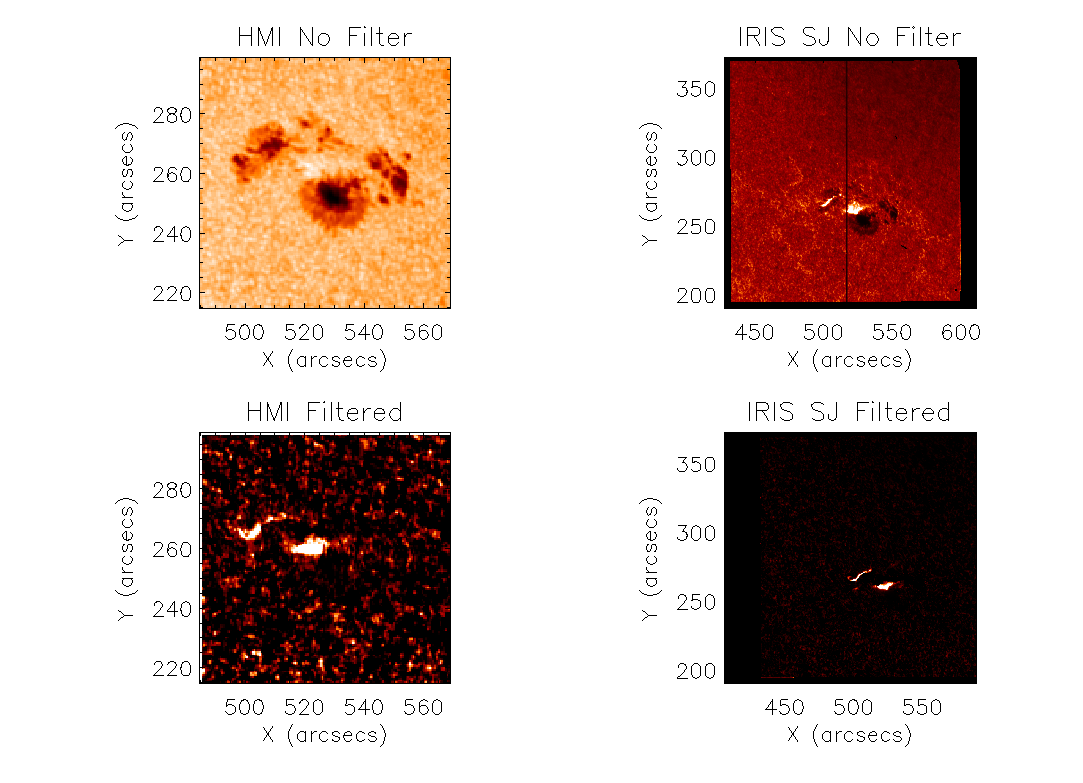
\includegraphics[width=0.8\textwidth]{29-Mar-14-diff-examples}
  \end{center}
  \caption{White light flares are difficult to observe against the bright photosphere requiring processing with a running difference filter to enhance ribbon features. The figure shows IRIS SJ 2832 \AA\ and SDO HMI continuum data before (top) and after (bottom) filtering.}\label{dif_filter}
\end{figure}

IRIS SJ and SG data are converted from relative intensity (DN per pixel) to energy (erg) units using conversion factors. Provided in the instrument documentation \citep{2014SoPh..289.2733D} is a method for acquiring the conversion factors in SSWIDL. It is then a case of inserting IRIS DN per pixel intensity values into the equation \ref{irisradiometriccal}. $F_{DN}$ is flux in units of DN per pixel, $C_{d2p}$ is the DN to photon conversion factor, $E_{\lambda}$ is the photon energy and $E_{erg}$ is to put the result into erg units.  

\begin{equation}\label{irisradiometriccal}
E = \frac{F_{DN}  C_{d2p} E_{\lambda}}{E_{erg}}
\end{equation}

To perform the same conversion for SDO HMI data required a slightly different approach due to the non-existent DN to photon conversion factor. Using a combination of sources \citep{2012SoPh..275...41B, 2012SoPh..275..285C} the instrument's properties are used to fulfil a conversion factor in the form of equation \ref{hmiradiometriccal}. Where $g$ is the instrument gain, $QE$ is the quantum efficiency of the charged couple device and $A_{ap}$ is the instrument aperture area, all other terms hold the same meaning as in equation \ref{irisradiometriccal}.

\begin{equation}\label{hmiradiometriccal}
E = \frac{F_{DN} E_{\lambda}}{g QE A_{ap} E_{erg}}
\end{equation}


For the IRIS and SDO HMI data sets, multiple sample points have been chosen based on locations specific to the sunquake and ribbon activity. Figures \ref{sirib}, \ref{mgrib}, \ref{mgwrib} and \ref{hmirib} show the ribbon coordinates sampled from each data set. Studying the flare in this way allows the energy distribution along the ribbon to be analysed and provides a point of comparison for the sunquake location. Each data set has five sample points per ribbon, a procedure which is repeated at two time frames, 17:45 and 17:46, providing twenty individual energy measurements per data set. The number of sample points will likely be increased in the future to provide better spatial resolution for ribbon energy distribution analysis. The problem with defining multiple ribbon samples over five different data sets comes when one considers the morphology of the local magnetic field. Accelerated charged material can only travel along the magnetic field, so the shape of those field lines will dictate the location of emission therefore the morphology of the ribbon. With this in mind the sample of coordinates chosen is based on matching common morphological features seen in each data set.

%insert figures showing ribbon coords oplot
\begin{figure}[H]
  \begin{center}
  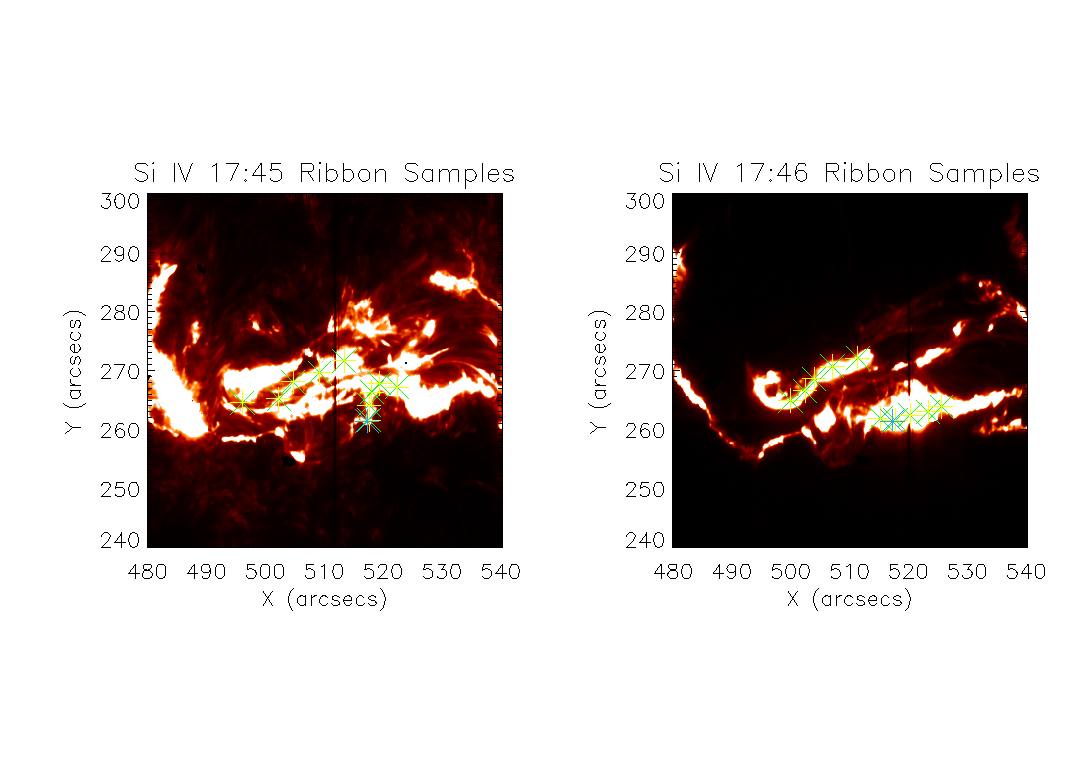
\includegraphics[width=0.8\textwidth]{29-Mar-14-SI-Ribbon-Coord-oplot}
  \end{center}
  \caption{Shows IRIS Si IV slit-jaw data with sampled ribbon and sunquake pixel coordinates marked in green and blue respectively. Twenty ribbon sample points are taken from two instances in time.}\label{sirib}
\end{figure}

\begin{figure}[H]
  \begin{center}
  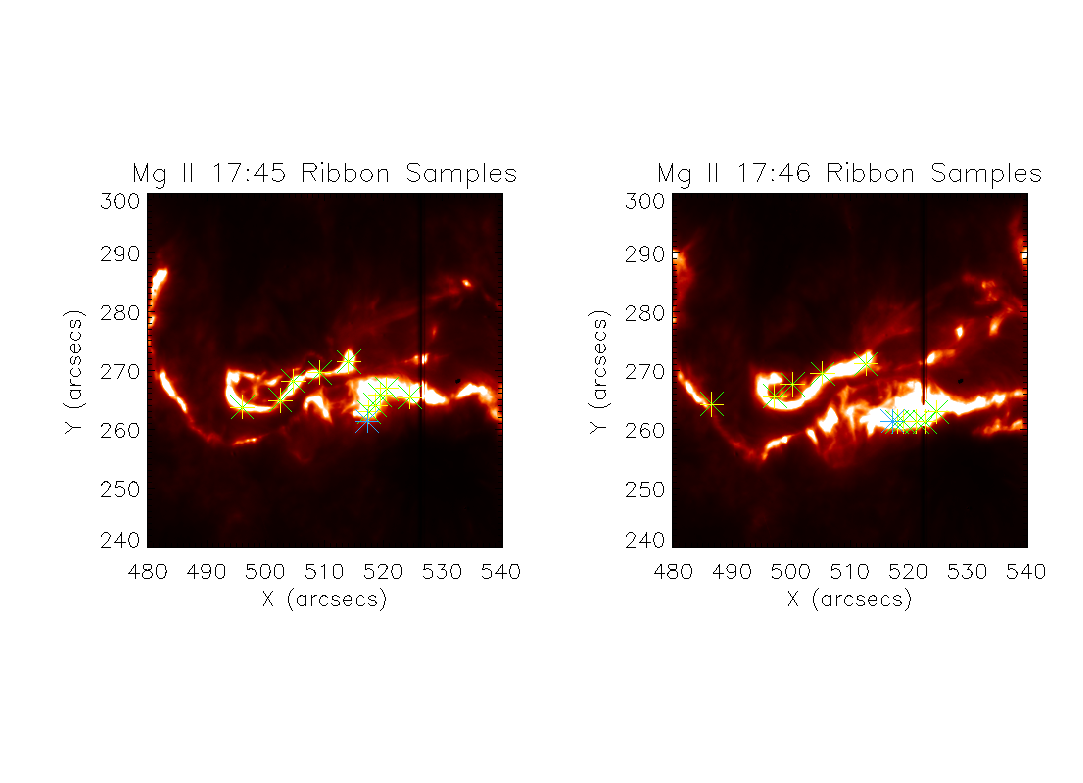
\includegraphics[width=0.8\textwidth]{29-Mar-14-MG-Ribbon-Coord-oplot}
  \end{center}
  \caption{Shows IRIS Mg II slit-jaw data with sampled ribbon and sunquake pixel coordinates marked in green and blue respectively. Twenty ribbon sample points are taken from two instances in time.}\label{mgrib}
\end{figure}

\begin{figure}[H]
  \begin{center}
  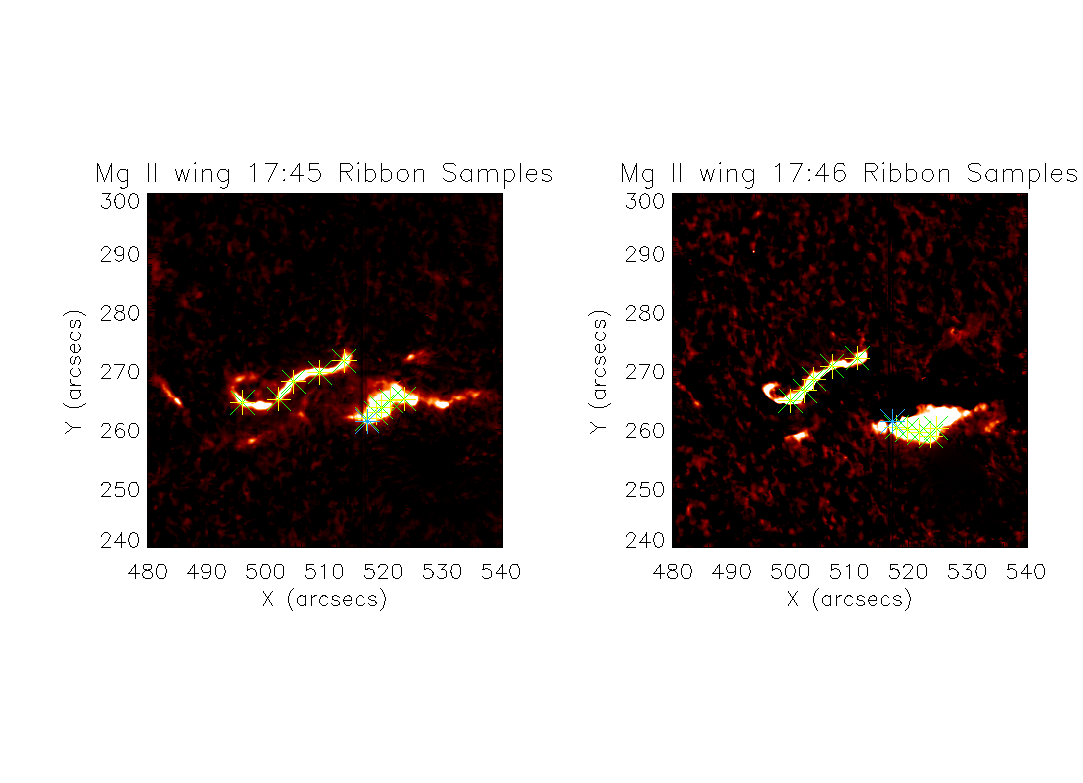
\includegraphics[width=0.8\textwidth]{29-Mar-14-MGW-Ribbon-Coord-oplot}
  \end{center}
  \caption{Shows IRIS Mg II wing slit-jaw data with sampled ribbon and sunquake pixel coordinates marked in green and blue respectively. Twenty ribbon sample points are taken from two instances in time.}\label{mgwrib}
\end{figure}

\begin{figure}[H]
  \begin{center}
  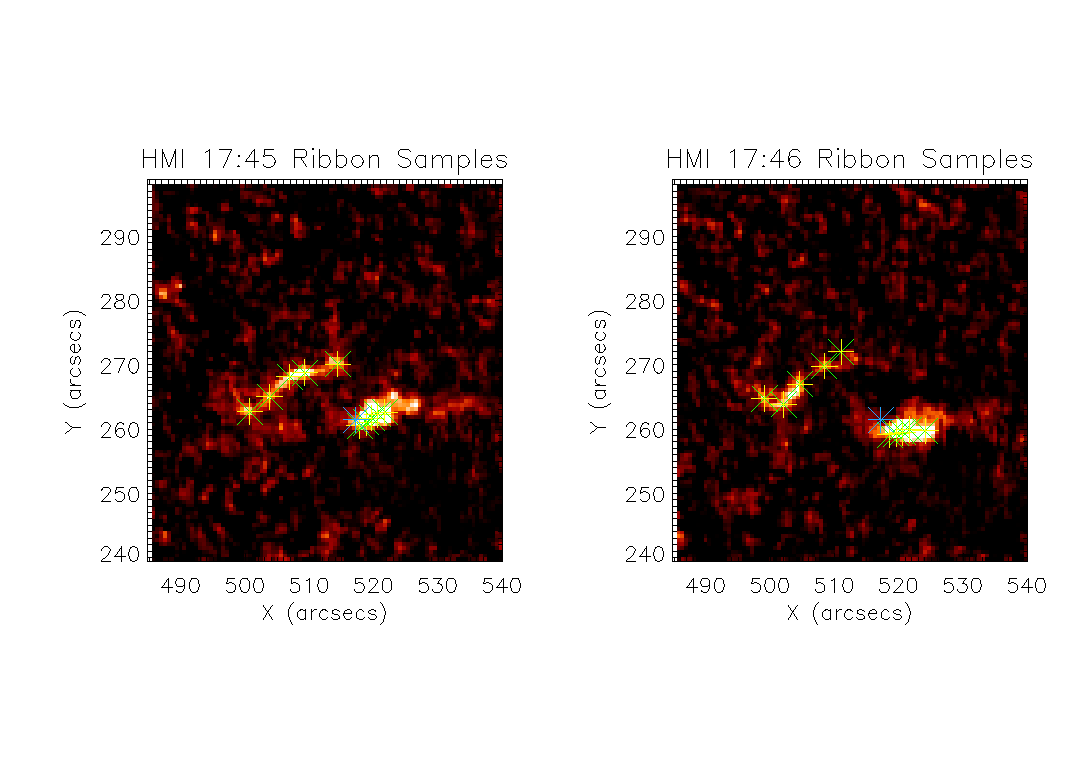
\includegraphics[width=0.8\textwidth]{29-Mar-14-HMI-Ribbon-Coord-oplot}
  \end{center}
  \caption{Shows SDO HMI continuum with sampled ribbon and sunquake pixel coordinates marked in green and blue respectively. Twenty ribbon sample points are taken from two instances in time. This procedure is also applied to IRIS SJ and SG data, see the Appendix for more figures.}\label{hmirib}
\end{figure}


IRIS spectroscopic data is sampled over a wavelength range of 2825.7 and 2825.8\AA\ (see \ref{balmercontinuum}) which is within the Balmer continuum. Balmer Data is sampled at slit positions and pixels that relate to one quake position and twenty ribbon samples, as with the other data sets. 

%insert figure showing balmer continuum spectrum sample range
\begin{figure}[H]
  \begin{center}
  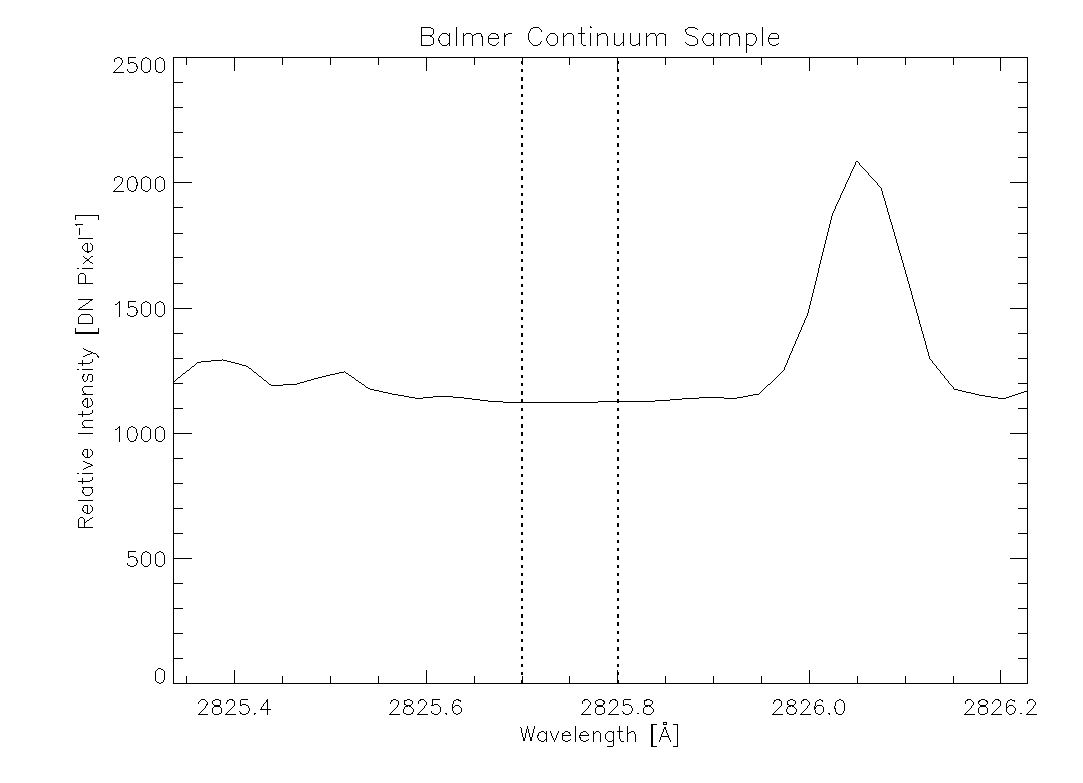
\includegraphics[width=0.8\textwidth]{29-Mar-14-Balmer-Continuum}
  \end{center}
  \caption{Shows the Balmer continuum component sampled from the IRIS SG data. Balmer emission is an indicator of radiative backwarming of the photosphere. }\label{balmercontinuum}
\end{figure}


Once all energies are calculated for each location and data set, time series energy-curves are created, see Figures \ref{erhessi} and \ref{eqk} (the Appendix contains the energy curves taken from ribbon locations). Each energy-time ladder plot contains energy curves from IRIS SJ 1400 \AA\, 2796 \AA\, SG Balmer, SJ 2832 \AA\ and SDO HMI continuum aligned in time. From top to bottom, the order of the plots in the ladder represents descending plasma temperature in the solar atmosphere see Tables \ref{iris-sg} and \ref{iris-sj}. Tables \ref{qkenergytab} and \ref{ribenergytab} display energy values taken from each pixel location and data set, except RHESSI, at two times corresponding to maximum WLF ribbon intensity at 17:45 and 17:46. Figure \ref{eqk} contains plots for the sunquake epicentre pixel, peak energies from each data set range from $9.63{\times}10^{14}$ erg from IRIS 1400 \AA\, $4.36{\times}10^{16}$ erg from IRIS 2796 \AA\ which is a lower limit due to over saturation of the instrument CCD, $2.68{\times}10^{16}$ erg from IRIS Balmer, $8.21{\times}10^{15}$ erg from IRIS 2832 \AA\ and $3.29{\times}10^{13}$ erg from SDO HMI continuum. 

\begin{figure}[H]
  \begin{center}
  \textbf{Quake Location Energy Over Time}\par\medskip
  \includegraphics[width=0.6\textwidth]{29-Mar-14-Quake-Energy-Ladder}
  \end{center}
  \caption{Shows calculated energy values over time of the region thought to be the sunquake epicentre (518.5", 264.0"). Each plot represents an independent data set, in order from top to bottom the sets are; IRIS SJ 1400 \AA\ (Si IV); IRIS SJ 2796 \AA\ (Mg II); IRIS SG  2825.7 to 2825.8 \AA\ (Balmer Continuum);IRIS SJ 2832 \AA\ (Mg II wing); SDO HMI continuum (HMI). The dotted line running vertically through each plot signifies a the onset time of the eruptive phase of the flare}\label{eqk}
\end{figure}

Ribbon plots show a wide range of properties. In an order dictated by Table \ref{ribenergytab}. The following is a bulletized summary of each ribbon position ladder-plot. The ribbon location is based on the HMI coordinates.

\begin{itemize}
\item Figure \ref{erb1} shows ribbon location 517.800, 260.500. Comparing peak energies from each data set to the sunquake pixel, this location shows; Si IV has 1.9 times more energy ; Mg II has 2 times more energy; Balmer has 0.47 of the energy; Mg II wing has 1.1 times more energy; HMI continuum has 2 times more energy. 

%less balmer seems to correspond with more hmi?    

\item Figure \ref{erb2} shows ribbon location 518.800, 261.000. Comparing peak energies from each data set to the sunquake pixel, this location shows; Si IV has 0.4 of the energy; Mg II has 0.65 of the energy; Balmer has 0.74 of the energy; Mg II wing has 1.03 times more energy; HMI continuum has 3.5 times more energy. 


\item Figure \ref{erb3} shows ribbon location 519.700, 261.700. Comparing peak energies from each data set to the sunquake pixel, this location shows; Si IV is saturated; Mg II is saturated; Balmer has 0.33 of the energy; Mg II wing has 2.8 times more energy; HMI continuum has 4.98 times more energy. 


\item Figure \ref{erb4} shows ribbon location 520.600, 262.300. Comparing peak energies from each data set to the sunquake pixel, this location shows; Si IV is saturated; Mg II has 0.36 of the energy; Balmer has 0.26 of the energy; Mg II wing has 0.94 of the energy; HMI continuum has 4.50 times more energy. 


\item Figure \ref{erb5} shows ribbon location 521.700, 262.600. Comparing peak energies from each data set to the sunquake pixel, this location shows; Si IV is saturated but shows at least 14.2 times more energy; Mg II is saturated; Balmer has 0.21 of the energy; Mg II wing has 1.08 times more energy; HMI continuum has 3.56 times more energy. 


\item Figure \ref{erb6} shows ribbon location 500.700, 262.700. Comparing peak energies from each data set to the sunquake pixel, this location shows; Si IV is saturated; Mg II is saturated; Balmer has 0.42 of the energy; Mg II wing has 0.72 of the energy; HMI continuum has 2.02 times more energy. 



\item Figure \ref{erb7} shows ribbon location 503.800, 265.000. Comparing peak energies from each data set to the sunquake pixel, this location shows; Si IV has 2.79; Mg II is saturated; Balmer has 0.21 of the energy; Mg II wing has 1.08 times more energy; HMI continuum has 3.56 times more energy. 



\item Figure \ref{erb8} shows ribbon location 506.900, 268.100. Comparing peak energies from each data set to the sunquake pixel, this location shows; Si IV is saturated; Mg II is saturated; Balmer has 0.13 of the energy; Mg II wing has 0.54 of the energy; HMI continuum has 2.40 times more energy. 


\item Figure \ref{erb9} shows ribbon location 509.277, 268.792. Comparing peak energies from each data set to the sunquake pixel, this location shows; Si IV is saturated; Mg II is saturated; Balmer has 0.07 of the energy; Mg II wing has 0.48 of the energy; HMI continuum has 3.04 times more energy. 


\item Figure \ref{erb10} shows ribbon location 514.400, 270.100. Comparing peak energies from each data set to the sunquake pixel, this location shows; Si IV is saturated; Mg II is saturated; Balmer has 0.12 of the energy; Mg II wing has 0.85 of the energy; HMI continuum has 1.5 times more energy. 


\item Figure \ref{erb11} shows ribbon location 518.600, 259.100. Comparing peak energies from each data set to the sunquake pixel, this location shows; Si IV has 2.50 times more energy; Mg II is saturated; Balmer has 0.82 of the energy; Mg II wing has 2.02 times more energy; HMI continuum has 1.68 times more energy. 


\item Figure \ref{erb12} shows ribbon location 519.600, 259.300. Comparing peak energies from each data set to the sunquake pixel, this location shows; Si IV has 0.5 of the energy; Mg II has 0.3 of the energy; Balmer has 1.01 times more energy; Mg II wing has 3.01 times more energy; HMI continuum has 2.51 times more energy. 


\item Figure \ref{erb13} shows ribbon location 520.600, 259.500. Comparing peak energies from each data set to the sunquake pixel, this location shows; Si IV has 2.3 times more energy; Mg II has 0.4 of the energy; Balmer has 1.80 times more energy; Mg II wing has 2.15 times more energy; HMI continuum has 3.77 times more energy.


\item Figure \ref{erb14} shows ribbon location 521.600, 259.900. Comparing peak energies from each data set to the sunquake pixel, this location shows; Si IV has 0.63 of the energy; Mg II has 0.28 of the energy; Balmer has 0.60 of the energy; Mg II wing has 2.37 times more energy; HMI continuum has 5.25 times more energy.



\item Figure \ref{erb15} shows ribbon location 524.100, 259.700. Comparing peak energies from each data set to the sunquake pixel, this location shows; Si IV is saturated; Mg II has 0.55 of the energy; Balmer has 1.26 times more energy; Mg II wing has 1.74 times more energy; HMI continuum has 3.27 times more energy.


\item Figure \ref{erb16} shows ribbon location 499.100, 264.700. Comparing peak energies from each data set to the sunquake pixel, this location shows; Si IV is saturated; Mg II has 0.15 of the energy; Balmer has 0.9 of the energy; Mg II wing has 2.84 times more energy; HMI continuum has 1.90 times more energy.


\item Figure \ref{erb17} shows ribbon location 502.100, 263.800. Comparing peak energies from each data set to the sunquake pixel, this location shows; Si IV is saturated; Mg II is saturated; Balmer has 0.72 of the energy; Mg II wing has 1.65 times more energy; HMI continuum has 2.32 times more energy.


\item Figure \ref{erb18} shows ribbon location 504.600, 267.000. Comparing peak energies from each data set to the sunquake pixel, this location shows; Si IV is saturated; Mg II is saturated; Balmer has 0.79 of the energy; Mg II wing has 2.11 times more energy; HMI continuum has 2.48 times more energy.



\item Figure \ref{erb19} shows ribbon location 508.400, 269.800. Comparing peak energies from each data set to the sunquake pixel, this location shows; Si IV is saturated; Mg II is saturated; Balmer has 0.41 of the energy; Mg II wing has 0.98 times more energy; HMI continuum has 1.71 times more energy.



\item Figure \ref{erb20} shows ribbon location 511.000, 272.000. Comparing peak energies from each data set to the sunquake pixel, this location shows; Si IV is saturated; Mg II is saturated; Balmer has 0.39 of the energy; Mg II wing has 0.67 of the energy; HMI continuum has 0.67 times more energy.
\end{itemize}

Another consideration is that Figure \ref{eqk} only relates to one pixel, therefore to analyse the energy emitted from an area comparable to the sunquake origin area would provide a better estimate of the radiative energy available. This has been calculated for HMI continuum data only, based on the sunquake area $2.6{\times}10^{16}$ $cm^{2}$ as stated in \cite{2014ApJ...796...85J}. Based on this area value 13 HMI pixels are sampled, summed and converted to energy, producing an upper limit of $2.54{\times}10^{17}$ erg. Comparing this to the sunquake energy, $1.3\pm0.05{\times}10^{26}$ $erg.s^{-1}$, also stated in \cite{2014ApJ...796...85J} to the hmi area estimate shows that the sunquake contains $10^{9}$ times more energy. 





\subsection{Results and Discussion}

This project presents a first look at a multi-wavelength energy analysis of the lower solar atmosphere during the 29th of March 2014 X class solar flare. The main focus up to this point has been to acquire energy estimates from the various atmospheric regions in an attempt to assess the likelihood of radiative backwarming as a generation method for the sunquake. The location of maximum acoustic power, RHESSI HXR, IRIS and SDO intensity correlate both spatially and temporally (see Figure \ref{saxcontours-vert}), showing that energy input into the upper chromosphere via accelerated non-thermal electrons propagates down to the photosphere. The sunquake is located directly underneath both maximum HXR and an area of white-light emission.

Energy estimates from RHESSI data show there to be between $1.0{\times}10^{28}$ to $2.5{\times}10^{29}$ erg during the impulsive phase of the flare. Comparing this to the sunquake energy of $1.3\pm0.05{\times}10^{26}$ $erg.s^{-1}$ means that the acoustic energy is well within the energy budget provided by accelerated non-thermal electrons, so how is the energy getting to the photosphere to cause seismic event?

Energy estimates from IRIS are not always useful due to over saturation of the instrument CCD, however, when comparing the ribbon locations to that of the sunquake some clear behaviours reveal themselves. The 1400 \AA\ channel is almost always showing greater radiative energy in all ribbon locations compared to the sunquake. This could be because transition region ribbons are rarely directly above the sunquake epicentre due to magnetic field configuration. The 2796 \AA\ channel becomes saturated slightly less often than the 1400 \AA\, providing more insight. The IRIS 2796 \AA\ channel is less in energy than the sunquake location around 30\% of the time. However, no real comparison can be attained due to the saturation of the CCD at the majority of ribbon pixels and the sunquake pixel. The only information that can be deduced, is that the sunquake pixel has an extraordinary 2796 \AA\ enhancement but then so do the majority of the ribbon locations. Balmer emission calculated from IRIS SG data is consistently of less energy than at the sunquake location, this is an interesting result as it means that there is more radiative backwarming above the sunquake pixel than in any other location sampled. However, the energy required to generate the sunquake is in the order of $10^25$ ergs, which when compared to the $2.68{\times}10^{16}$ erg of energy available in the Balmer pixel is $10^{9}$ times greater! Perhaps radiative backwarming only plays a bit-part in the generation of the sunquake?  
The 2832 \AA\ IRIS channel is harder to summarise due to the fact that comparing ribbon locations to that of the sunquake show that there is a 50:50 chance that the ribbon could have greater or lower energy output.
SDO HMI continuum data is probably the most revealing, in that almost all of the ribbon locations have far greater energy output than the sunquake location. This could be explained by the sunquake being only partially under a white light ribbon. 

In conclusion, this analysis has barely scratched the surface of the information available in the data. Some immediate trends have been noticed such as the lower levels of Balmer and higher levels of photospheric continuum energy in the flare ribbons compared to the sunquake. Is there a connection between these two emission regions, and do these signatures have anything to do with the generation of the sunquake? In general the data sets available are tending to show that there is not enough energy in atmospheric emission to generate the sunquake via radiative backwarming.

  

\subsection{Future Work}
Obviously there is a need for a much more detailed analysis, which will be the main task for the immediate future. Plotting energy behaviours of each ribbon location and data set would help to visualise the trends discussed. There is plans to analyse $\gamma$-ray and magnetogram data to look for signatures associated with direct particle collision and impulsive magnetic field reconfiguration respectively. IRIS SG data will be used to analyse Doppler-shift to look for shock waves.

\subsubsection{In the Last Few Months}
The majority of the work carried out since the last panel meeting has been:
\begin{itemize}
\item Calculate energy associated with emission captured by HMI to compare with the acoustic power of the sunquake.
\item Calculate energy associated with emission captured by IRIS slit jaw and spectrometer in order to estimate energy deposition in the atmosphere.
\item Calculate energy associated with Balmer emission to assess likely energy contribution of radiative backwarming.
\item Calculate non-thermal electron power via HXR spectra to estimate the initial energy of the electron beam accelerated by the corona.
\end{itemize}




%%%%%%%%%%%%%%%%%%%%%%%%%%%%%%\include{projectupgrd-rewrite}
%%%%%%%%%%%%%%%%%%%%%%%%%%%%%%\appendix
\appendixpage
\addappheadtotoc
%
% \begin{figure}%[H]
%   \begin{center}
%   \includegraphics[width=0.8\textwidth]{}
%   \end{center}
%   \caption{Left panel shows data over the quake location, right panel shows data over the ribbon location. From top to bottom, plots show lightcurves from IRIS Si IV, Mg II, Balmer wavelengths and Mg II wing, with the bottom panel showing the lightcurve from SDO HMI.}\label{lcseries-bold}
% \end{figure}
\section{Ribbon Pixel Coordinates}\label{ribcoords}
%insert figure showing ribbon coords oplot
\begin{figure}%[H]
  \begin{center}
  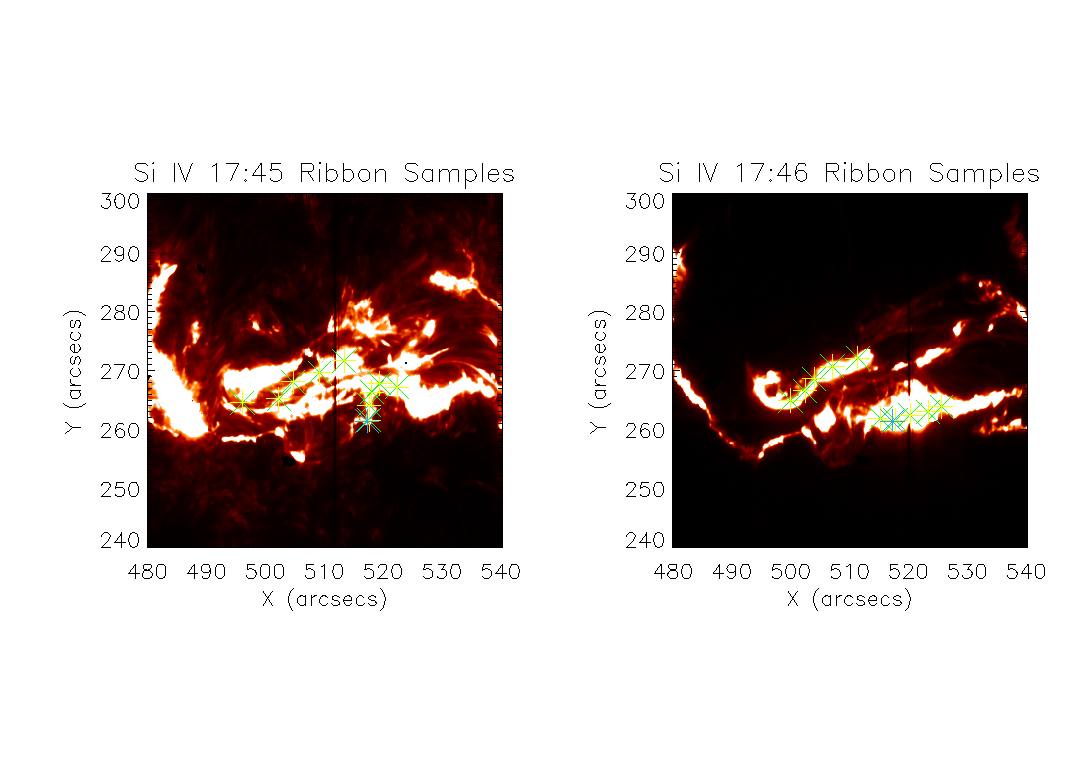
\includegraphics[width=0.8\textwidth]{29-Mar-14-SI-Ribbon-Coord-oplot}
  \end{center}
  \caption{Shows IRIS Si IV slit-jaw data with sampled ribbon and sunquake pixel coordinates marked in green and blue respectively. Twenty ribbon sample points are taken from two instances in time.}\label{sirib}
\end{figure}

\begin{figure}%[H]
  \begin{center}
  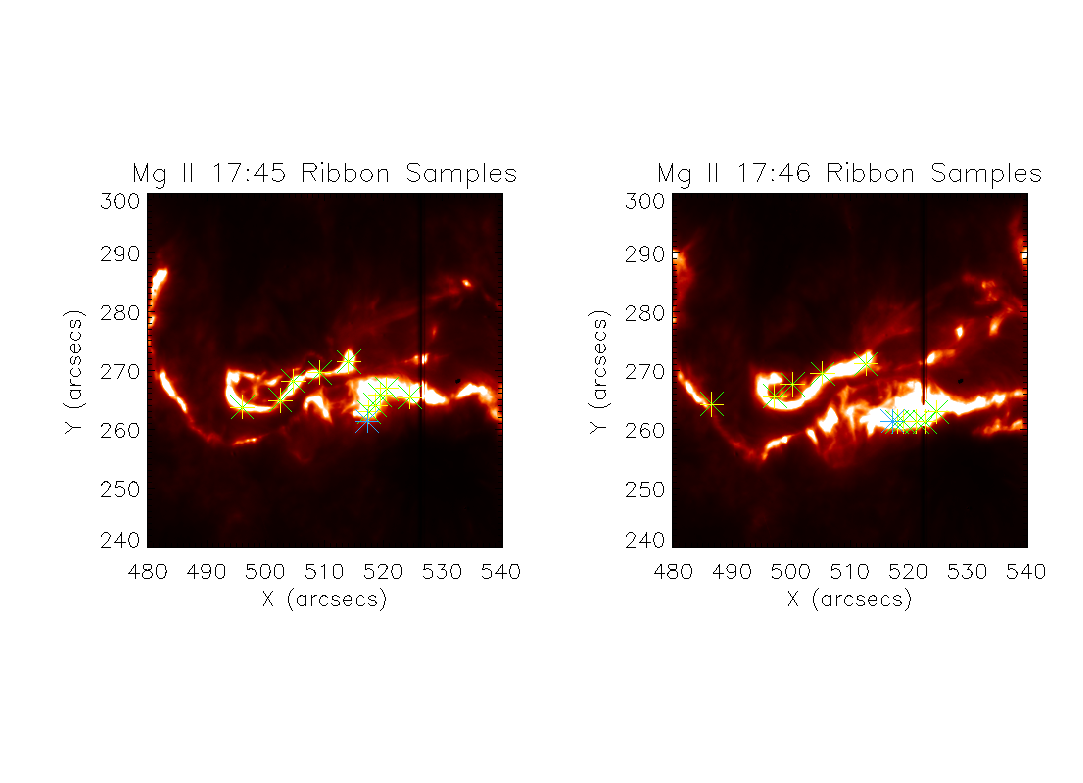
\includegraphics[width=0.8\textwidth]{29-Mar-14-MG-Ribbon-Coord-oplot}
  \end{center}
  \caption{Shows IRIS Mg II slit-jaw data with sampled ribbon and sunquake pixel coordinates marked in green and blue respectively. Twenty ribbon sample points are taken from two instances in time.}\label{mgrib}
\end{figure}

\begin{figure}%[H]
  \begin{center}
  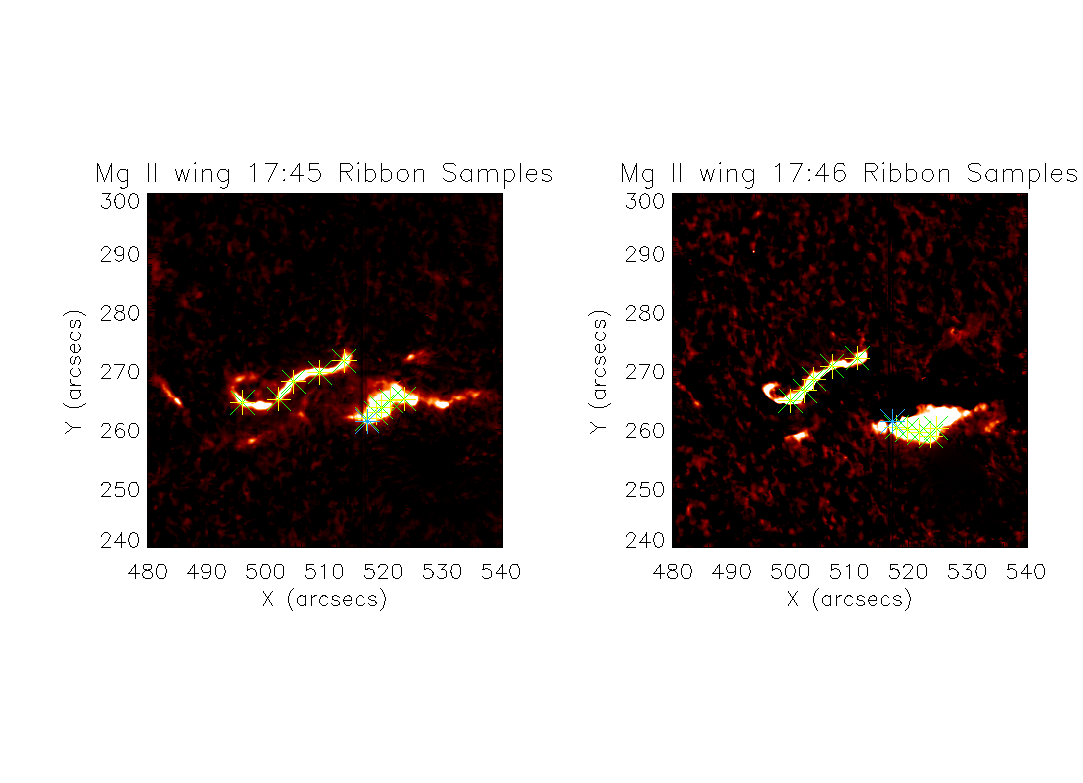
\includegraphics[width=0.8\textwidth]{29-Mar-14-MGW-Ribbon-Coord-oplot}
  \end{center}
  \caption{Shows IRIS Mg II wing slit-jaw data with sampled ribbon and sunquake pixel coordinates marked in green and blue respectively. Twenty ribbon sample points are taken from two instances in time.}\label{mgwrib}
\end{figure}

\appendix
\appendixpage
\addappheadtotoc
%
% \begin{figure}%[H]
%   \begin{center}
%   \includegraphics[width=0.8\textwidth]{}
%   \end{center}
%   \caption{Left panel shows data over the quake location, right panel shows data over the ribbon location. From top to bottom, plots show lightcurves from IRIS Si IV, Mg II, Balmer wavelengths and Mg II wing, with the bottom panel showing the lightcurve from SDO HMI.}\label{lcseries-bold}
% \end{figure}

%insert figure showing ribbon coords oplot
%\graphicspath{ {~/PhD/Thesis/upgrade-plots/}}


%contains energy time plots for quake and ribbon locations
%also contains energy tables


%\includegraphics[trim=left bottom right top, clip]{file}
\section{Equations}\label{mhdeqns}
\paragraph{Maxwell's Equations and Ohm's Law}
Maxwell's equations and Ohm's law describe electromagnetism in terms of magnetic induction $\vec{B}$, magnetic permeability of free space $\mu$, electric field $\vec{E}$, electrical permittivity of free space $\epsilon_{0}$, charge density $\rho_{c}$ and electric current density $\vec{j}$ \\ 

\textbf{Ampère's Law}
\begin{equation}\label{max1:ampere}
\nabla\times\vec{B}=\mu_{0}(\vec{j}+\epsilon_{0}\frac{\partial \vec{E}}{\partial t})
\end{equation}

\textbf{Faraday's Law}
\begin{equation}\label{max2:faraday}
\nabla\times\vec{E}=-\frac{\partial \vec{B}}{\partial t}
\end{equation}

\textbf{Gauss's Law}
\begin{equation}\label{max3:gauss}
\nabla\cdot\vec{E}=\frac{\rho_{c}}{\epsilon_{0}}
\end{equation}

\textbf{No Magnetic Monopoles}
\begin{equation}\label{max4:nomonopole}
\nabla\cdot\vec{B}=0
\end{equation}

with Ohm's law as,

\begin{equation}\label{ohmslaw}
\vec{j}=\sigma(\vec{E}+\vec{v}\times\vec{B})
\end{equation}

where $\sigma$ is electrical conductivity. 

\paragraph{Fluid Dynamics Equations}
The fluid dynamics relations are written in terms of density $\rho$, velocity $\vec{v}$, time $t$, pressure $p$, gas constant $\Re$ and temperature $T$. 
%$\frac{d}{dt}=\frac{\partial}{\partial t}+ \vec{v}\cdot\nabla$, sometimes reffered to as the material derivative, is a way of stating the rate of change with respect to time of the  

\begin{equation}\label{motion}
\rho\frac{d\vec{v}}{dt}=-\nabla p
\end{equation}
 
\begin{equation}\label{masscontinuity}
\frac{d\rho}{dt}+\rho\nabla\cdot\vec{v}=0
\end{equation}

\begin{equation}\label{perfectgaslaw}
p=\Re\rho T
\end{equation}

Equation \ref{motion} is the eqn. of motion describing how the forces are exerted on the fluid are equal to the negative gradient of plasma pressure. Equation \ref{masscontinuity} is the eqn. of mass continuity (mass is conserved), whilst equation \ref{perfectgaslaw} is the perfect gas law relating plasma pressure, density and temperature. 

\paragraph{MHD Equations}
Another way to write the relationship between $\vec{B}$ and $\vec{v}$ is the equation of motion \ref{motion} modified by the Lorentz force.

\begin{equation}\label{motion1}
\rho\frac{d\vec{v}}{dt}=-\nabla p+\vec{j}\times\vec{B}
\end{equation}

The pressure gradient $-\nabla p$ describes the change from high to low plasma pressure. The Lorentz force, $\vec{j}\times\vec{B}$ acts perpendicularly to the magnetic field, therefore accelerated plasma in a direction parallel to the magnetic field is caused by other forces. If equation \ref{new1} is substituted into the Lorentz force,
\begin{equation}\label{lorentzsub1}
\vec{j}\times\vec{B} = (\nabla\times\frac{\vec{B}}{\mu})\times\vec{B}
\end{equation}


\begin{equation}\label{maghydstat}
\rho\frac{d\vec{v}}{dt}= -\nabla p + (\vec{B}\cdot\nabla)\frac{\vec{B}}{\mu}-\nabla(\frac{B^2}{2\mu}) 
\end{equation}

Because $-\nabla(\frac{B^2}{2\mu}$ is in the same form as $-\nabla p$ it can be said to be the \emph{magnetic pressure}, providing a force pointing from high to low magnetic pressure as $B^2$ changes with position.

\paragraph{Reduced MHD Equations}
Based on assumptions:
\begin{itemize}
\item $v<<v_{c}$, typical plasma velocities are much slower than the sound speed 
\item All the effects of radiation, viscosity, electric charge density and displacement currents are negligable 
\end{itemize}
It is possible to reduce Maxwell's equations into the following form:

\textbf{Ampère's Law}
\begin{equation}\label{max1:ampere}
\nabla\times\vec{B}=\mu_{0}\vec{j}
\end{equation}

\textbf{Faraday's Law}
\begin{equation}\label{max2:faraday}
\nabla\times\vec{E}=-\frac{\partial \vec{B}}{\partial t}
\end{equation}

\textbf{Gauss's Law}
\begin{equation}\label{max3:gauss}
\nabla\cdot\vec{E}=0
\end{equation}

\textbf{No Magnetic Monopoles}
\begin{equation}\label{max4:nomonopole}
\nabla\cdot\vec{B}=0
\end{equation}

\section{Figures}\label{figures}

\begin{figure}[H]
  \begin{center}
  \includegraphics[width=0.6\textwidth]{29-Mar-14-Ribbon-Area-1-Sunquake-Area-Power-Ladder}
  \end{center}
  \caption{Shows radiative power from an area comparable to the sunquake impact, centered on region 1, relating to heliocentric coordinates 518.2", 262.0" which is directly over the sunquake location. Each plot represents an independant data set, in order from top to bottom the sets are; IRIS SJ 1400 \AA\ (Si IV); IRIS SJ 2796 \AA\ (Mg II); IRIS SG  2825.7 to 2825.8 \AA\ (Balmer Continuum); IRIS SJ 2832 \AA\ (Mg II wing); SDO HMI continuum (HMI).}\label{plot1}
\end{figure}
\begin{figure}[H]
  \begin{center}
  \textbf{Quake Location Energy Over Time}\par\medskip
  \includegraphics[width=0.6\textwidth]{29-Mar-14-Ribbon-Area-2-Sunquake-Area-Power-Ladder}
  \end{center}
  \caption{Shows radiative power from an area comparable to the sunquake impact, centered on region 2, which relates to heliocentric coordinates 520.2", 263.0". Each plot represents an independant data set, in order from top to bottom the sets are; IRIS SJ 1400 \AA\ (Si IV); IRIS SJ 2796 \AA\ (Mg II); IRIS SG  2825.7 to 2825.8 \AA\ (Balmer Continuum); IRIS SJ 2832 \AA\ (Mg II wing); SDO HMI continuum (HMI).}\label{plot2}
\end{figure}


\begin{figure}[H]
  \begin{center}
  \textbf{Quake Location Energy Over Time}\par\medskip
  \includegraphics[width=0.6\textwidth]{29-Mar-14-Ribbon-Area-3-Sunquake-Area-Power-Ladder}
  \end{center}
  \caption{Shows radiative power from an area comparable to the sunquake impact, centered on region 3, which relates to heliocentric coordinates 522.2", 262.0". Each plot represents an independant data set, in order from top to bottom the sets are; IRIS SJ 1400 \AA\ (Si IV); IRIS SJ 2796 \AA\ (Mg II); IRIS SG  2825.7 to 2825.8 \AA\ (Balmer Continuum); IRIS SJ 2832 \AA\ (Mg II wing); SDO HMI continuum (HMI).}\label{plot3}
\end{figure}

\begin{figure}[H]
  \begin{center}
  \textbf{Quake Location Energy Over Time}\par\medskip
  \includegraphics[width=0.6\textwidth]{29-Mar-14-Ribbon-Area-4-Sunquake-Area-Power-Ladder}
  \end{center}
  \caption{Shows radiative power from an area comparable to the sunquake impact, centered on region 4, which relates to heliocentric coordinates 522.2", 265.0". Each plot represents an independant data set, in order from top to bottom the sets are; IRIS SJ 1400 \AA\ (Si IV); IRIS SJ 2796 \AA\ (Mg II); IRIS SG  2825.7 to 2825.8 \AA\ (Balmer Continuum); IRIS SJ 2832 \AA\ (Mg II wing); SDO HMI continuum (HMI).}\label{plot4}
\end{figure}

\begin{figure}[H]
  \begin{center}
  \textbf{Quake Location Energy Over Time}\par\medskip
  \includegraphics[width=0.6\textwidth]{29-Mar-14-Ribbon-Area-5-Sunquake-Area-Power-Ladder}
  \end{center}
  \caption{Shows radiative power from an area comparable to the sunquake impact, centered on region 5, which relates to heliocentric coordinates 524.3", 265.0". Each plot represents an independant data set, in order from top to bottom the sets are; IRIS SJ 1400 \AA\ (Si IV); IRIS SJ 2796 \AA\ (Mg II); IRIS SG  2825.7 to 2825.8 \AA\ (Balmer Continuum); IRIS SJ 2832 \AA\ (Mg II wing); SDO HMI continuum (HMI).}\label{plot5}
\end{figure}

\begin{figure}[H]
  \begin{center}
  \textbf{Quake Location Energy Over Time}\par\medskip
  \includegraphics[width=0.6\textwidth]{29-Mar-14-Ribbon-Area-6-Sunquake-Area-Power-Ladder}
  \end{center}
  \caption{Shows radiative power from an area comparable to the sunquake impact, centered on region 6, which relates to heliocentric coordinates 526.3", 263.8". Each plot represents an independant data set, in order from top to bottom the sets are; IRIS SJ 1400 \AA\ (Si IV); IRIS SJ 2796 \AA\ (Mg II); IRIS SG  2825.7 to 2825.8 \AA\ (Balmer Continuum); IRIS SJ 2832 \AA\ (Mg II wing); SDO HMI continuum (HMI).}\label{plot6}
\end{figure}

%\include{appendix-rewrite}

\label{Bibliography}
\lhead{\emph{Bibliography}}  % Change the left side page header to "Bibliography"
%\bibliographystyle{unsrtnat}  % Use the "unsrtnat" BibTeX style for formatting the Bibliography
\bibliographystyle{plainnat}%abbrv}
\bibliography{../Bibliography/Bibliography}  % The references (bibliography) information are stored in the file named "Bibliography.bib"
%\bibliography{Bibliography}
\end{document}
